\documentclass[11pt]{article}

% ---------- packages ----------
\usepackage[utf8]{inputenc}
\usepackage[T1]{fontenc}
\usepackage{lmodern}
\usepackage[strings]{underscore}   % lets literal "_" appear in text/tables without escaping
\usepackage[margin=1in]{geometry}
\usepackage{amsmath,amssymb,amsfonts}
\usepackage{booktabs}
\usepackage{array}
\usepackage{tabularx}
\usepackage{longtable}
\usepackage{multirow}
\usepackage{graphicx}
\usepackage{xcolor}
\usepackage{tikz}
\usetikzlibrary{arrows.meta, positioning, shapes.geometric, fit, calc}
\usepackage{listings}
\usepackage{caption}
\usepackage{enumitem}
\usepackage[colorlinks=true, linkcolor=blue!50!black, citecolor=blue!50!black, urlcolor=blue!50!black]{hyperref}
\usepackage{titling}

\lstset{
  basicstyle=\ttfamily\small,
  breaklines=true,
  columns=fullflexible,
  frame=single,
  backgroundcolor=\color{gray!5},
  commentstyle=\color{gray!60!black},
  keywordstyle=\color{blue!60!black},
  numbers=none
}

\newcolumntype{Y}{>{\raggedright\arraybackslash}X}

\newcommand{\placeholderfig}[2]{%
\begin{figure}[h]
\centering
\fbox{\begin{minipage}{0.88\textwidth}
\centering\vspace{1.4cm}
\textit{[PLACEHOLDER --- #1]}
\vspace{1.4cm}
\end{minipage}}
\caption{#2}
\end{figure}
}

\title{\Large Phase 1: Conceptual Mapping (Deconstruction)\\[4pt]
\large Reproduction of \emph{Bioacoustic classification of avian calls from raw sound
waveforms with an open-source deep learning architecture}\\
(Bravo Sanchez, Hossain, English \& Moore, \emph{Sci.\ Rep.} 11, 15733, 2021),\\
on the NIPS4Bplus dataset (Morfi, Bas, Pamu\l{}a, Glotin \& Stowell, 2019),\\
architecturally descended from SincNet (Ravanelli \& Bengio, 2018)}
\author{}
\date{}

\begin{document}
\maketitle

\begin{abstract}
\noindent This document is the Phase 1 deliverable --- Conceptual Mapping
(Deconstruction) --- for a from-scratch reproduction of the SincNet-based
avian bioacoustic classifier described above, run against the authors' own
companion code and the released NIPS4Bplus corpus. It covers three required
parts: (A) Problem Formulation, grounded in a full exploratory data analysis
of the raw corpus rather than the papers' stated summary statistics; (B)
Methodological Justification, a layer-by-layer, hyperparameter-by-hyperparameter
mathematical dissection of the training pipeline as it is actually configured
in the tracked \texttt{.cfg} files (not as idealized in the paper's prose);
and (C) Data Pipeline Analysis, an algorithmic breakdown of preprocessing,
missing-value handling, feature scaling, and class-imbalance handling, with a
theoretically-justified redesign discussion. Every statistic below was either
measured directly from the 687 raw training files and 674 annotation CSVs on
disk, or read directly from the executable training/config code --- not
transcribed from the papers' text without verification. Figures 1--15 are
generated directly from that raw data; Figure 16 is a closed-form illustrative
plot of the SincConv filter's own mathematical definition. Three explicit
placeholders mark diagrams that require information (GPS metadata, a trained
model's learned filter weights, hardware photographs) not obtainable from the
released data alone.
\end{abstract}

\tableofcontents
\newpage

% ======================================================================
\section{Part A --- Problem Formulation}
% ======================================================================

\subsection{The problem, in ML terms}
\label{sec:A1}

Stripped of domain language, the paper solves:

\begin{quote}
\itshape Given a short window of a raw acoustic waveform known to contain an
animal vocalisation, predict which of $C$ discrete, mutually exclusive
classes produced it.
\end{quote}

Formally, the model is a parametric function
\[
f_\theta : \mathbb{R}^{w} \to \Delta^{C-1}
\]
mapping a fixed-length raw-amplitude window $\mathbf{x}\in\mathbb{R}^{w}$
($w=$ \texttt{wlen}, in samples) to a point on the $(C-1)$-simplex --- a
categorical probability distribution over $C$ classes --- via
\[
f_\theta(\mathbf{x}) = \operatorname{softmax}\big(g_\theta(\mathbf{x})\big),
\qquad
\hat y = \arg\max_{c\in\{1,\dots,C\}} f_\theta(\mathbf{x})_c .
\]

This is \textbf{single-label, multi-class classification} on a
\textbf{fixed-length, raw, univariate time-series input} --- not sequence
labelling / detection (the model is never asked to decide \emph{where} in a
longer recording a call starts; that segmentation is given by the
human-annotated \texttt{start}/\texttt{length} fields), not regression, not
multi-label (\texttt{class\_act=softmax}, \texttt{cost = NLLLoss()} --- a
single label per window, not a set), and not self-supervised representation
learning (there is no pretext task; every layer trains directly against the
ground-truth species label from epoch 1).

\subsection{Target variable(s)}
\label{sec:A2}

The repository defines \textbf{three separate target-variable schemes} over
the same underlying event table, corresponding to three separately-trained
models (the \texttt{class\_lay} field of each config):

\begin{table}[h]
\centering
\begin{tabularx}{\textwidth}{l c Y}
\toprule
Scheme (config file) & $C$ & What one integer label encodes \\
\midrule
All Classes  & 87 & \texttt{<species-or-insect-or-amphibian>\_<call\_type>} --- call/song/drum kept as distinct classes \\
Bird Classes & 77 & same, restricted to \texttt{type == 'bird'} \\
Bird Species & 51 & bird species only, with call/song/drum \textbf{merged} into one label per species (grouped by \texttt{Scientific} name, not \texttt{Class}) \\
\bottomrule
\end{tabularx}
\end{table}

The label itself is an \textbf{integer index assigned by first-appearance
order} in \texttt{pandas.unique()} over the (unordered) file list
(\texttt{generate\_mod\_file\_lists.py}) --- i.e.\ the label$\to$integer
mapping is an artifact of list-generation order, not a stable, semantically
meaningful ID (see Section~\ref{sec:A7}). The distribution of the target
variable itself (class imbalance) is quantified in Section~\ref{sec:A54}.

\subsection{Input feature space}
\label{sec:A3}

This is the single most consequential design decision in the paper, and it
inverts the usual ``feature engineering'' framing: \textbf{there is no
engineered feature vector.} The input is the raw waveform itself,
\[
\mathbf{x} = [x_0, x_1, \dots, x_{w-1}], \qquad x_i \in [-1,1]\ \text{(post peak-normalisation)},
\]
a window of $w=$ \texttt{wlen} $=\lfloor f_s \cdot cw\_len / 1000\rfloor$
consecutive PCM samples at $f_s = 44{,}100$ Hz (measured directly from every
wav header, Table~\ref{tab:corpus}). For the enhanced Bird-Species/Bird-Classes
config, $cw\_len=16$~ms $\Rightarrow w=705$; for All Classes, $cw\_len=18$~ms
$\Rightarrow w=794$; for the default/Part-I config, $cw\_len=10$~ms
$\Rightarrow w=441$.

There is exactly \textbf{one derived scalar computed before the model sees
the data}: the per-file peak-normalisation divisor $\max(\text{signal})$
(Section~\ref{sec:C3}). Everything else --- spectral content, timbre,
pitch-like structure --- is left for the network's first layer (SincConv,
Section~\ref{sec:B33}) to discover. This is an explicit rejection of the
conventional bioacoustic pipeline
\[
\text{waveform} \to \text{STFT} \to |X(t,f)| \to \text{MFCC/Mel} \to \text{classifier},
\]
motivated (per the paper, and independently corroborated by the duration
statistics of Section~\ref{sec:A53}) by the concern that hand-designed
spectral features import assumptions from human-speech processing (Mel
scale, frame lengths tuned for phonemes) that do not necessarily transfer to
non-human bioacoustic signals.

\subsection{Learning paradigm}
\label{sec:A4}

\textbf{Supervised.} Every training example is a (window, label) pair; the
label comes from a human annotator's temporal-annotation CSV, not from any
self- or weak-supervision signal. It is not reinforcement learning (no
reward, no environment, no sequential decision process) and not unsupervised
(no clustering/density-estimation objective anywhere in \texttt{call\_id.py};
the only unsupervised-\emph{flavoured} component is that the Sinc filters'
cutoff frequencies are Mel-initialised before supervised fine-tuning --- an
initialisation scheme, not a training objective; Section~\ref{sec:B33}).

Within supervised learning it is specifically:
\begin{itemize}[nosep]
\item \textbf{discriminative}, not generative ($P(y\mid x)$ is modelled
  directly via \texttt{LogSoftmax}, never $P(x\mid y)$ or $P(x,y)$);
\item \textbf{frame/window-level} during training, with \textbf{file-level
  aggregation} at evaluation time via $\hat c = \arg\max_c \sum_t \log P_t(c)$
  (Section~\ref{sec:A6});
\item \textbf{closed-set}: $C$ is fixed at training time (87/77/51); there is
  no ``none of the above''/open-set rejection mechanism, even though roughly
  a third of the raw recordings contain no tagged event at all.
\end{itemize}

\subsection{Exploratory data analysis}
\label{sec:A5}

\subsubsection{What ``the dataset'' actually is, before any modelling choice}
\label{sec:A51}

\begin{table}[h]
\centering
\caption{The raw corpus, measured directly from the wav/CSV files on disk.}
\label{tab:corpus}
\begin{tabularx}{\textwidth}{Y c c}
\toprule
 & train (used for modelling) & test / 2013-challenge pool (unused) \\
\midrule
wav files & 687 & 1{,}000 \\
total duration & 2{,}903.2 s (48.4 min) & 4{,}172.5 s (69.5 min) \\
sample rate / channels / bit depth & 44{,}100 Hz / mono / \textbf{16-bit PCM} (paper states 32-bit) & same \\
files with $\geq 1$ tagged event & 569 & n/a --- no labels exist \\
files confirmed empty (reviewed, nothing found) & 105 & n/a \\
files with no annotation record at all & 13 & n/a \\
raw tag rows parsed & 5{,}775 & --- \\
tag rows after dropping \texttt{Unknown}/\texttt{Human} & 5{,}481 (paper: 5{,}478, after also dropping 3 sub-10ms events) & --- \\
\bottomrule
\end{tabularx}
\end{table}

The two populations (``687 labelled train files'' vs.\ ``1{,}000-file
\texttt{test/} folder'') are \textbf{not} the train/test split the models are
actually scored against --- that split is instead carved by
\texttt{train\_test\_split(..., stratify=..., test\_size=0.25)} out of the
687-file pool's \emph{tags}, three times independently, once per class
scheme (Section~\ref{sec:A7}, Section~\ref{sec:B4}). A two-sample
Kolmogorov--Smirnov comparison of the 687- vs.\ 1{,}000-file \emph{raw
corpora} (not the modelling split) shows RMS energy, zero-crossing rate,
spectral centroid, bandwidth, and flatness all differ significantly at
$\alpha=0.01$ (see Figure~\ref{fig:13}), while duration, crest factor, and
silence ratio do not.

\begin{figure}[h]
\centering
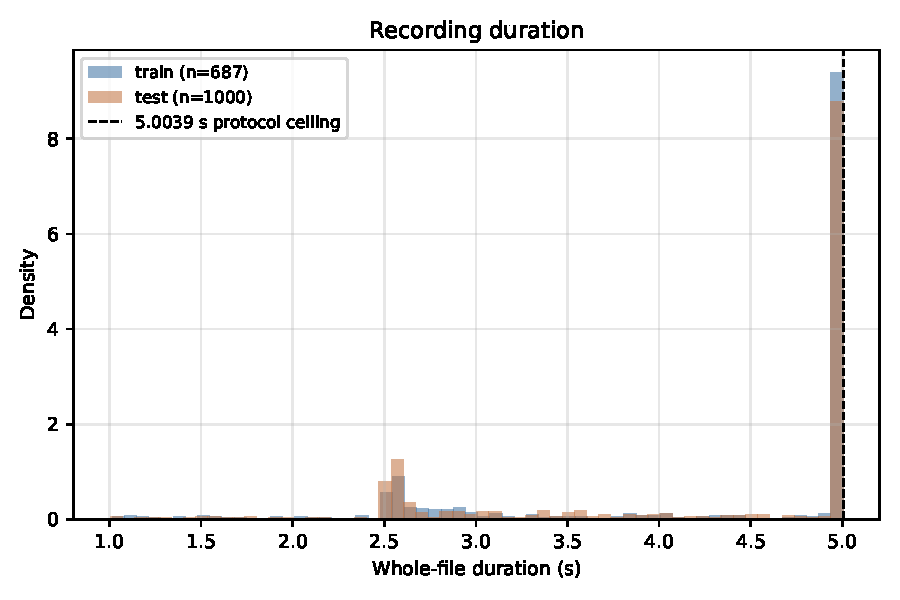
\includegraphics[width=0.85\textwidth]{figures/01_file_duration_hist.pdf}
\caption{File-duration histogram, train vs.\ test pool. File duration is a
censored mixture, not a smooth continuous variable: 61.9\% of train files sit
exactly at the 5.0039~s collection ceiling.}
\label{fig:01}
\end{figure}

\begin{figure}[h]
\centering
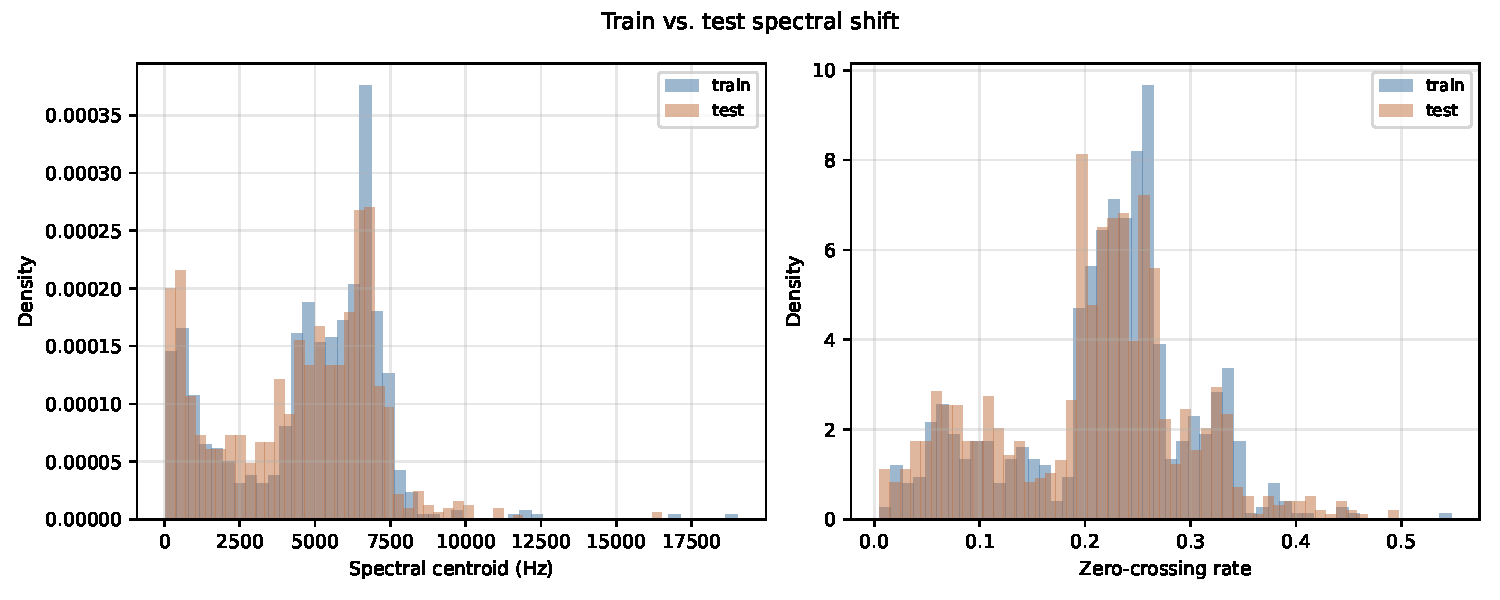
\includegraphics[width=0.8\textwidth]{figures/13_train_test_shift.pdf}
\caption{Two-sample KS comparison of whole-file features, 687-file train
pool vs.\ 1{,}000-file unused test pool. Amplitude-shape statistics
(duration, crest factor, silence ratio) are statistically indistinguishable
between the two pools; every spectral statistic (RMS, ZCR, centroid,
bandwidth, flatness) shows a significant shift at $\alpha=0.01$.}
\label{fig:13}
\end{figure}

\placeholderfig{insert a map of the 7 recording regions (Haute-Loire,
Pyr\'en\'ees-Orientales/Aude/H\'erault, Granada/Ja\'en/Almer\'ia) with the
20\%/65\%/15\% sampling-share breakdown, per Morfi et al.\ (2019), Fig.~1. Not
reproducible from the released audio/annotation files alone --- no per-file
GPS metadata ships with the dataset release.}{Placeholder --- geographic
sampling distribution of recording sites (source: Morfi et al.\ 2019, Fig.~1;
not independently verifiable from the released files).}

\subsubsection{Whole-file waveform statistics --- shape, not just mean/variance}
\label{sec:A52}

File duration is \textbf{not} a smooth random variable (Figure~\ref{fig:01})
--- the collection protocol (``split anything longer than 5~s into 5-s
chunks'') produces a censored mixture: most files pile up at the ceiling, the
rest are the tail-end remainder of a longer recording. Fitting a single
Gaussian/lognormal to file duration is fitting the wrong generative model; it
is reported descriptively only (mean 4.226~s, median 5.004~s, std 1.150~s,
skew $-1.09$).

\begin{table}[h]
\centering
\caption{Amplitude- and spectrum-domain descriptive statistics, train ($n=687$).}
\label{tab:waveform-stats}
\small
\begin{tabular}{l r r r r l}
\toprule
Feature & mean & std & skew & exc.\ kurt.\ & best-fit family (AIC-ranked) \\
\midrule
RMS energy               & 0.00352 & 0.02969 & 22.4 & 545 & \textbf{Lognormal} ($\Delta$AIC$=469$) \\
Crest factor (peak/RMS)  & 8.28    & 8.97    & 9.13 & 115 & \textbf{Lognormal} ($\Delta$AIC$=1{,}218$) \\
Dynamic range (dB)       & 16.86   & 4.23    & 1.76 & 5.95 & --- \\
Silence ratio            & 0.324   & 0.190   & 0.60 & 0.11 & --- \\
Zero-crossing rate       & 0.219   & 0.085   & $-0.42$ & 0.21 & --- \\
Spectral centroid (Hz)   & 4{,}770 & 2{,}516 & $-0.06$ & 1.40 & Weibull (barely; $\Delta$AIC$=28$ vs.\ Normal) \\
Spectral bandwidth (Hz)  & 4{,}355 & 1{,}614 & $-0.55$ & $-0.72$ & Weibull (barely; $\Delta$AIC$=109$ vs.\ Normal) \\
Spectral flatness        & 0.245   & 0.153   & $-0.15$ & $-1.42$ & --- \\
\bottomrule
\end{tabular}
\end{table}

\textbf{Formal normality is rejected for every feature} (Shapiro--Wilk and
D'Agostino $K^2$, $p<10^{-13}$), in both raw and log form --- but with
$n=687$ this is expected: these tests have enough statistical power to
detect any non-zero higher moment, so rejection here is a statement about
sample size, not practical effect size. The informative signal is the
\emph{magnitude} of skew/kurtosis (Table~\ref{tab:waveform-stats}) and which
parametric family minimises AIC --- this report treats ``what shape is it''
as the right question, not ``is it normal.''

RMS energy and crest factor are \textbf{unambiguously lognormal} by a wide
AIC margin --- the theoretically expected shape for a quantity produced by
many multiplicative, roughly-independent attenuating/amplifying factors
(source loudness, distance, atmospheric absorption, microphone gain),
consistent with the multiplicative Central Limit Theorem:
\[
f_{\text{lognormal}}(x;\mu,\sigma)=\frac{1}{x\sigma\sqrt{2\pi}}
\exp\!\left(-\frac{(\ln x-\mu)^2}{2\sigma^2}\right),\quad x>0 .
\]
Spectral centroid/bandwidth, being \emph{averages over many frequency bins},
are pulled back toward near-Gaussian shape regardless of the underlying bin
distribution --- Weibull edges out Normal only marginally.

\begin{figure}[h]
\centering
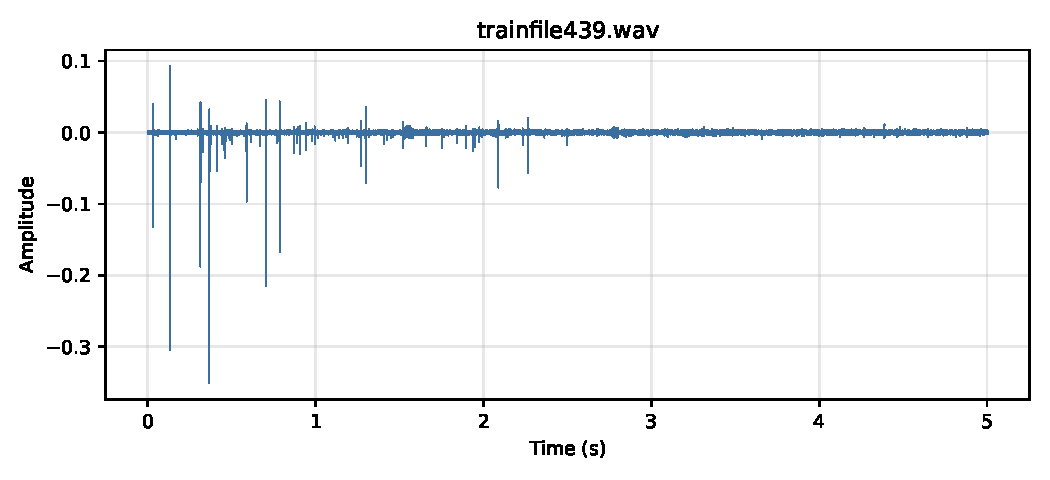
\includegraphics[width=0.75\textwidth]{figures/14_amplitude_outlier_trainfile439.pdf}
\caption{\texttt{nips4b\_birds\_trainfile439.wav}: crest factor $150\times$,
excess kurtosis 5{,}453 --- an order of magnitude beyond the next most
extreme file. A single sharp transient in an otherwise near-silent
recording. Illustrates why mean $\pm$ std summaries of amplitude features in
this dataset are misleading; median/IQR or a log transform is the honest
summary.}
\label{fig:14}
\end{figure}

\begin{figure}[h]
\centering
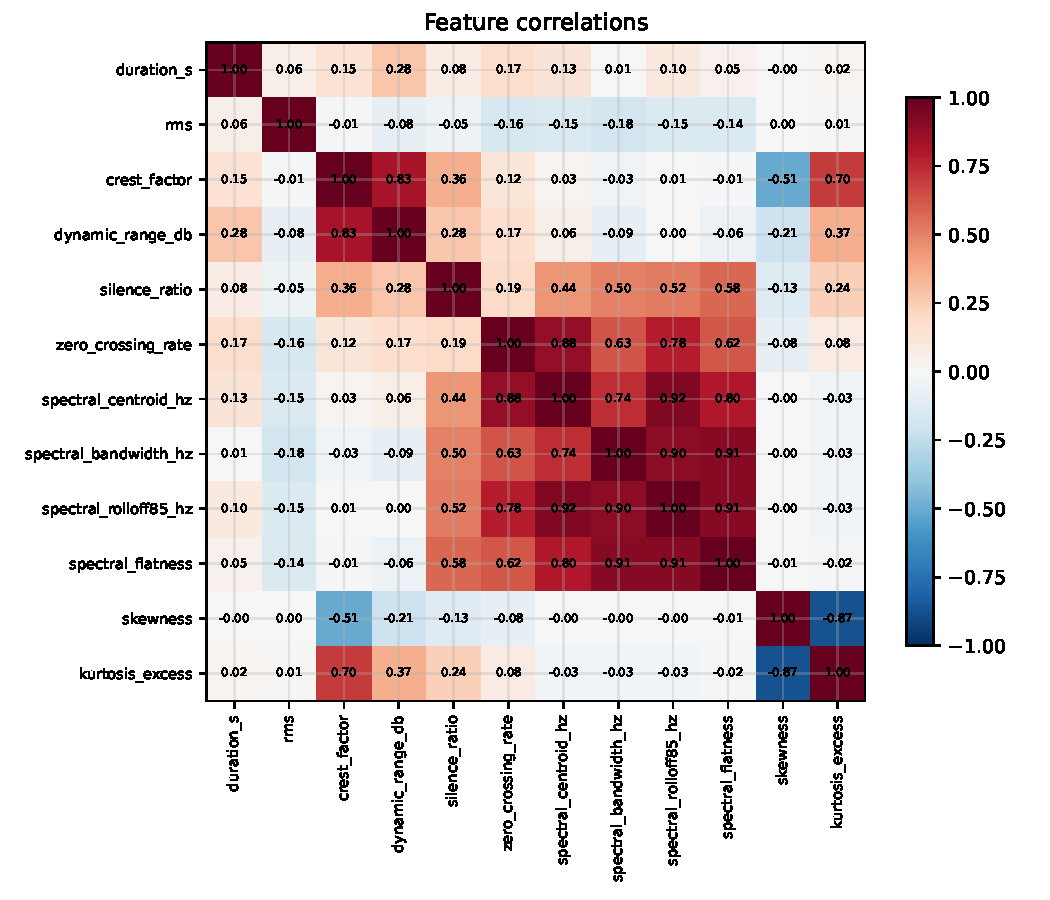
\includegraphics[width=0.8\textwidth]{figures/11_correlation_heatmap.pdf}
\caption{Correlation structure of whole-file features. Three clusters:
timbre/spectral-shape ($r=0.6$--$0.92$: ZCR, centroid, bandwidth, rolloff,
flatness), impulsiveness (crest factor $\leftrightarrow$ dynamic range,
$r=0.83$; skew $\leftrightarrow$ kurtosis, $r=-0.87$), and silence ratio
bridging both ($r=0.44$--$0.58$ with the spectral cluster).}
\label{fig:11}
\end{figure}

\begin{figure}[h]
\centering
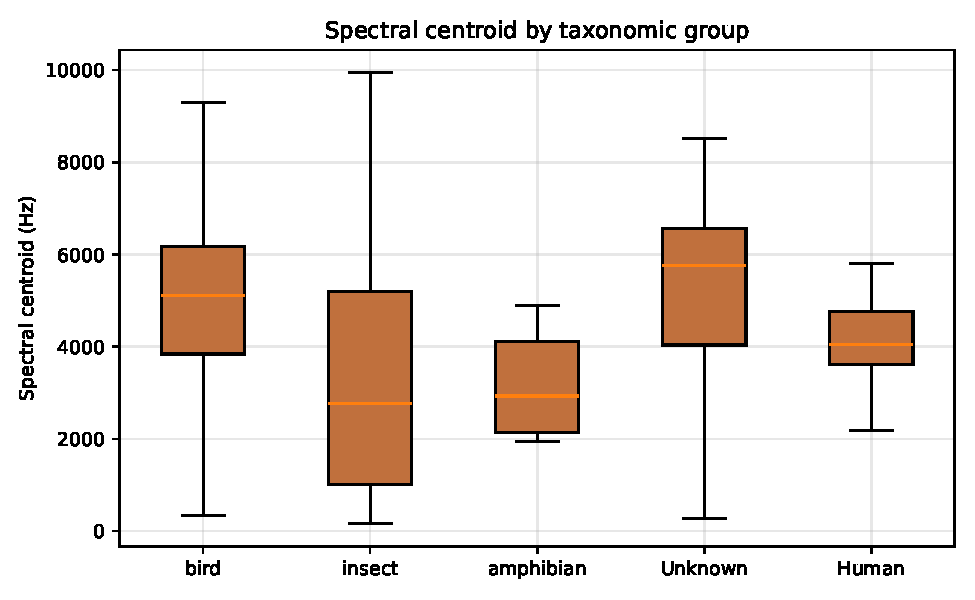
\includegraphics[width=0.75\textwidth]{figures/12_spectral_centroid_by_taxon.pdf}
\caption{Spectral centroid by taxon (event-level, exact tagged segment).
Insects register a visibly higher median spectral centroid than birds ---
consistent with cicada/bush-cricket stridulation concentrating energy in a
narrow high-frequency band. \texttt{Plaaff\_song} tops the 87-class table at
7{,}180~Hz mean centroid; the lowest is \texttt{Hirrus\_call} at 896~Hz.}
\label{fig:12}
\end{figure}

\subsubsection{Tagged-event duration --- the motivating EDA finding}
\label{sec:A53}

This is the single statistical fact that most directly justifies the paper's
central architectural choice (shrinking the analysis window from
speech-scale 200~ms to 10--18~ms):

\begin{table}[h]
\centering
\caption{Tagged-event duration by taxon.}
\label{tab:event-duration}
\begin{tabular}{l r r r r}
\toprule
 & all events ($n{=}5{,}775$) & bird ($n{=}5{,}279$) & insect ($n{=}168$) & amphibian ($n{=}34$) \\
\midrule
mean     & 0.195 s & 0.149 s & 1.670 s & 0.228 s \\
median   & 0.090 s & 0.087 s & 1.033 s & 0.192 s \\
std      & 0.455   & 0.220   & 1.775   & 0.203   \\
skewness & 7.29    & 5.14    & 0.78    & 3.33    \\
range    & 23~$\mu$s--5.00 s & 23~$\mu$s--2.78 s & 25 ms--5.00 s & 28 ms--1.19 s \\
\bottomrule
\end{tabular}
\end{table}

\begin{figure}[h]
\centering
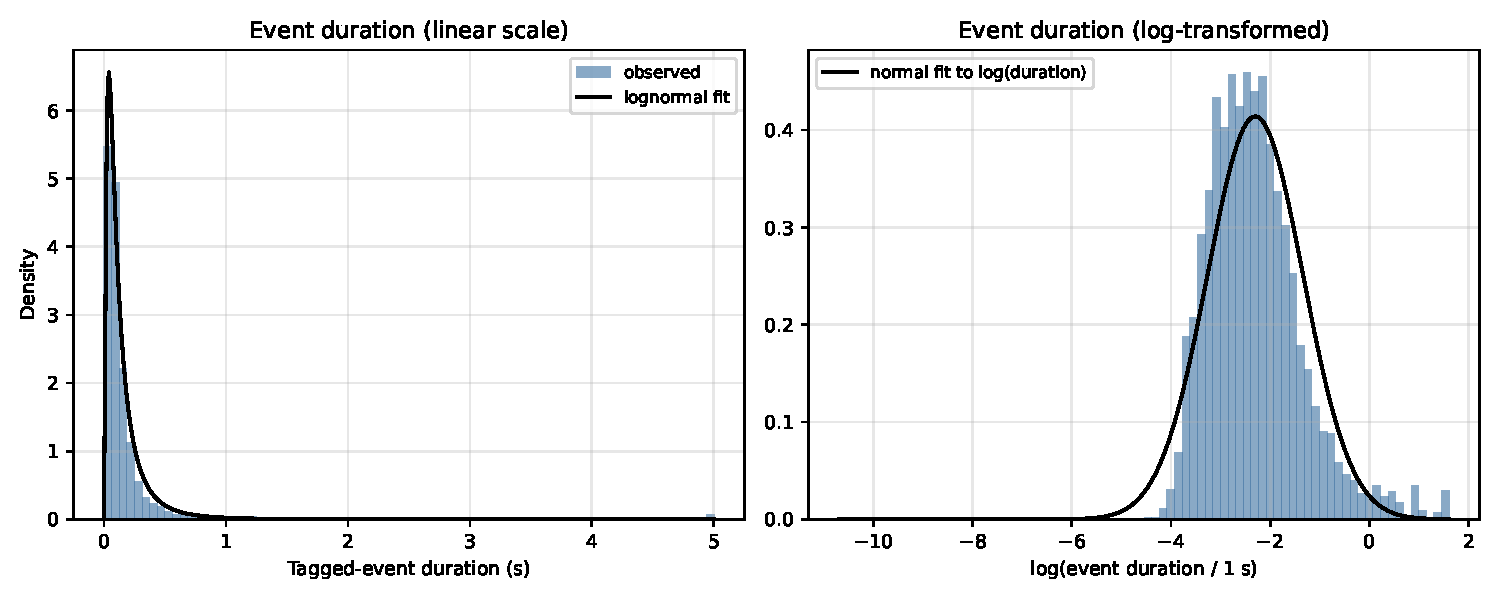
\includegraphics[width=0.75\textwidth]{figures/02_event_duration_distribution.pdf}
\caption{Tagged-event duration distribution, all 5{,}775 events. Best-fit
family: lognormal, by a wide margin ($\Delta$AIC $>3{,}200$), fitted
$\sigma\approx0.96$, scale $\approx0.10$~s.}
\label{fig:02}
\end{figure}

\begin{figure}[h]
\centering
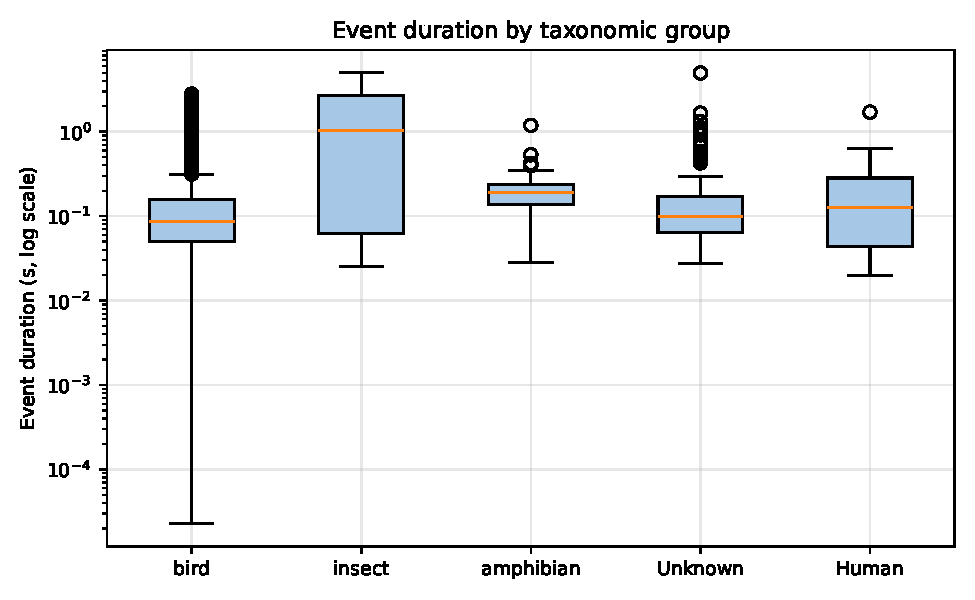
\includegraphics[width=0.75\textwidth]{figures/03_event_duration_by_taxon.pdf}
\caption{Event duration by taxon. Insects are the one exception to the
lognormal rule: with only 168 samples and a spread that mixes brief
stridulation bursts with long sustained calls, Gamma edges out Lognormal.}
\label{fig:03}
\end{figure}

\begin{figure}[h]
\centering
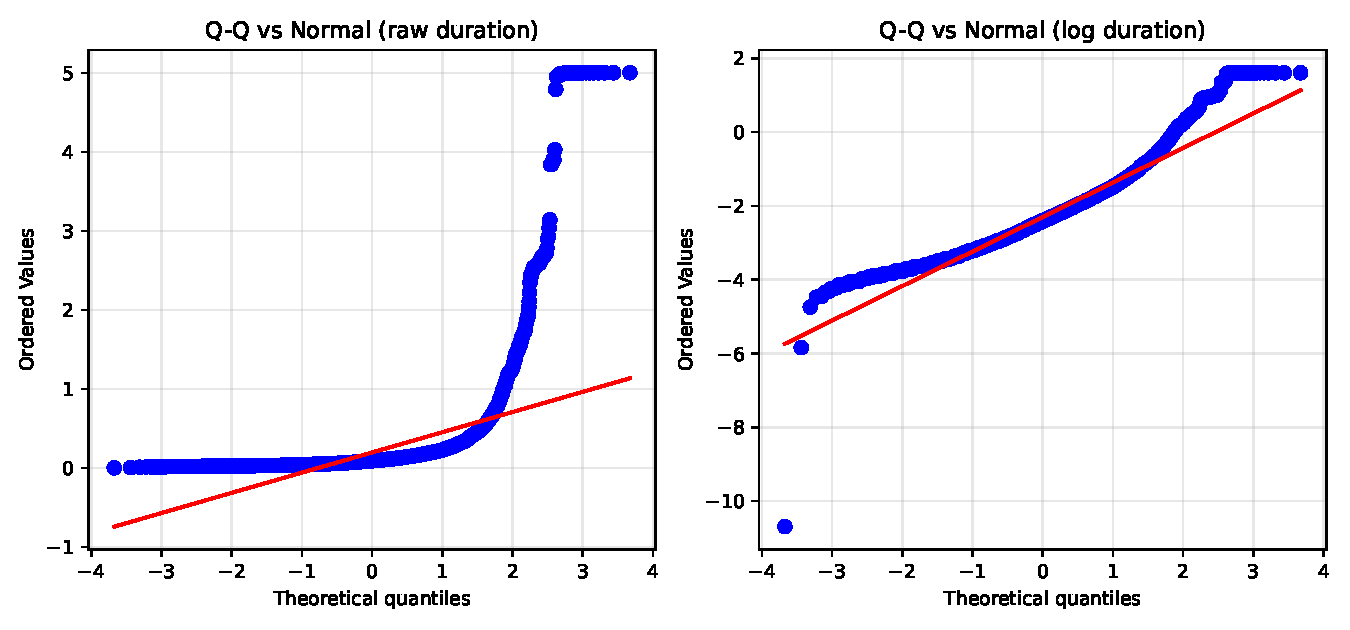
\includegraphics[width=0.7\textwidth]{figures/04_qq_event_duration.pdf}
\caption{Q--Q plot, log-transformed event duration vs.\ Normal quantiles.
Log-transforming turns a distribution unusable for Gaussian-based reasoning
into one that visually passes.}
\label{fig:04}
\end{figure}

The practical reading of a right-skewed, lognormal duration distribution:
\textbf{the typical call is much shorter than the mean call}, because a thin
tail of very long songs pulls the mean up over $2\times$ above the median ---
exactly the situation where designing a window length around the mean,
rather than the bulk of the probability mass, would be a mistake.

Quantitatively: only \textbf{14 of 5{,}775 events (0.24\%)} are shorter than
the enhanced pipeline's own window (16~ms for bird schemes, 18~ms for
all-classes), and only \textbf{3 (0.05\%)} are at or under 10~ms --- exactly
the ``three very short files\ldots which could not be processed without code
modifications'' the paper's methods section references, and the precise
reason \texttt{call\_id.py}'s windowing function needs the
shorter-than-window branch described in Section~\ref{sec:B32}.

Independent cross-checks against the paper's own reported per-class numbers
(computed with no reference to the paper's text, then compared afterward)
land within rounding: shortest-mean class \texttt{Sylcan\_call} measured at
31.1~ms (paper: ``$\sim$30~ms''), longest-mean class \texttt{Plasab\_song}
at 4.674~s (paper: ``more than 4.5~s''), most/least frequent classes match
exactly.

\subsubsection{Class imbalance --- the target variable's own distribution}
\label{sec:A54}

\[
\text{Gini} = \frac{2\sum_{i=1}^{n} i\,x_{(i)}}{n\sum_i x_i} - \frac{n+1}{n},
\qquad
H = -\sum_i p_i\log_2 p_i,
\qquad
N_{\text{eff}} = 2^{H}
\]
where $x_{(i)}$ are class counts sorted ascending and $p_i=x_i/\sum_i x_i$.
$N_{\text{eff}}$ (``effective number of classes'') is the count of
\emph{equally frequent} classes that would produce the same entropy.

\begin{table}[h]
\centering
\caption{Class-imbalance metrics.}
\label{tab:imbalance}
\begin{tabular}{l c c c c c c c}
\toprule
Scheme & classes & min/max & max/min & Gini & entropy (bits) & $N_{\text{eff}}$ & Zipf slope ($R^2$) \\
\midrule
All Classes  & 87 & 9/282  & $31.3\times$ & 0.447 & 5.967 & 62.5 (72\%) & $-0.84$ (0.88) \\
Bird Classes & 77 & 12/282 & $23.5\times$ & 0.426 & 5.839 & 57.2 (74\%) & $-0.80$ (0.88) \\
\bottomrule
\end{tabular}
\end{table}

\begin{figure}[h]
\centering
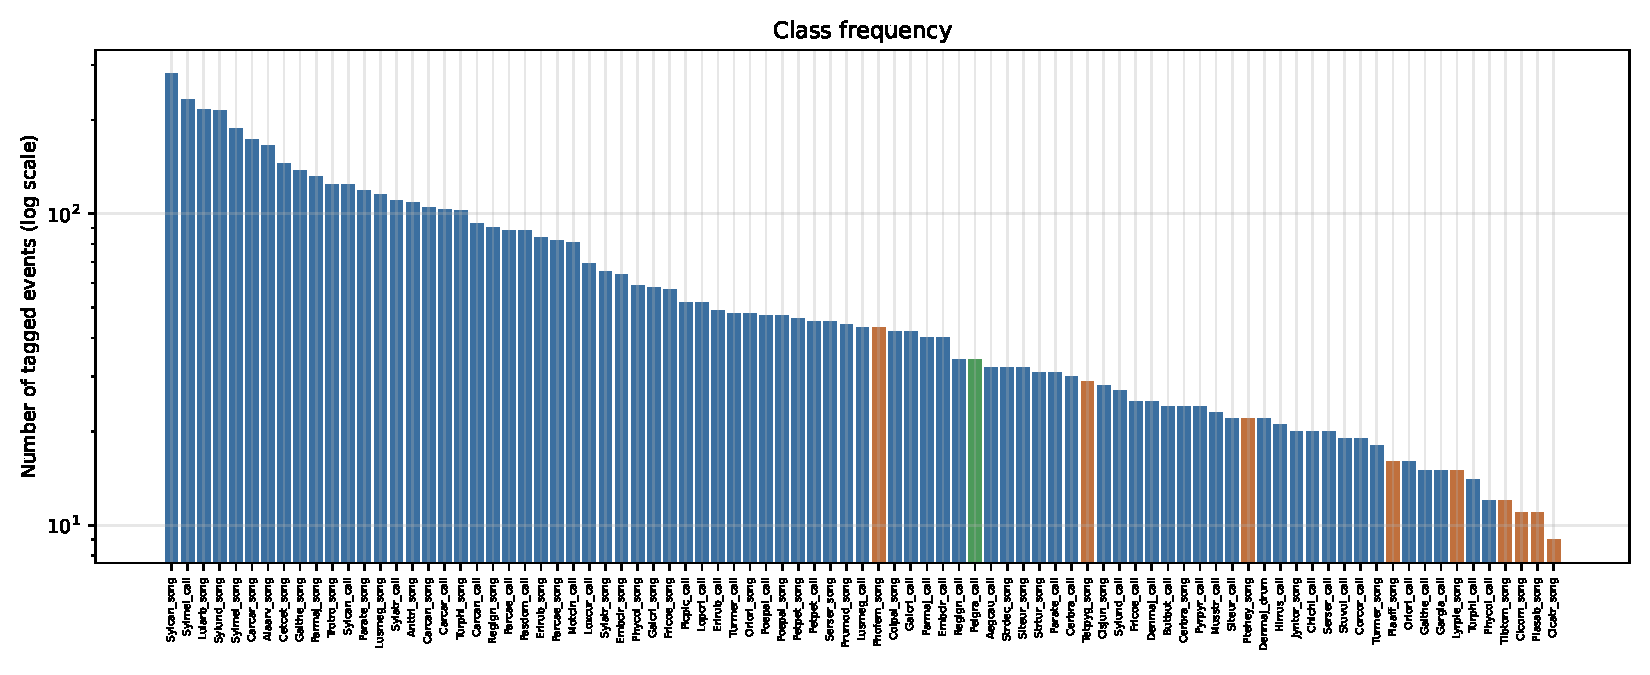
\includegraphics[width=0.75\textwidth]{figures/05_class_frequency.pdf}
\caption{Class frequency, log scale, All Classes (87).}
\label{fig:05}
\end{figure}

\begin{figure}[h]
\centering
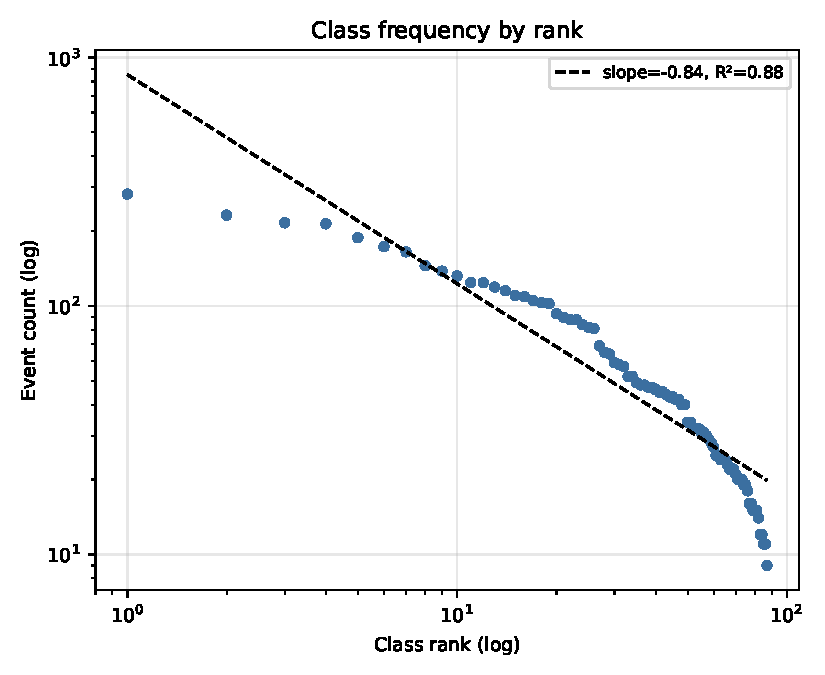
\includegraphics[width=0.7\textwidth]{figures/06_zipf_plot.pdf}
\caption{Zipf plot: class frequency decays roughly as $\text{rank}^{-1}$
($R^2\approx0.88$) --- between near-uniform and catastrophically long-tailed.}
\label{fig:06}
\end{figure}

\begin{figure}[h]
\centering
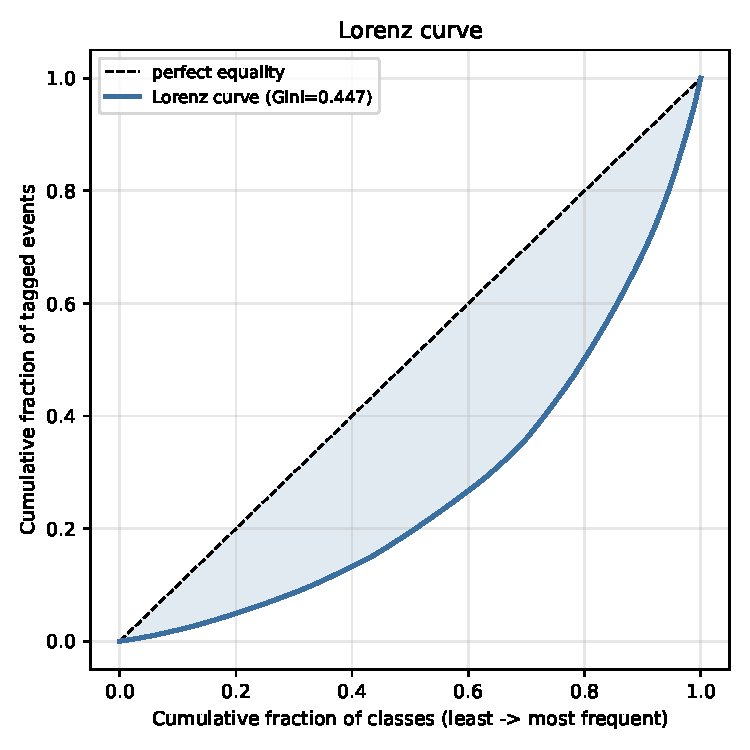
\includegraphics[width=0.7\textwidth]{figures/07_lorenz_curve.pdf}
\caption{Lorenz curve: the least-frequent half of the 87 classes account for
only $\sim$19\% of all tagged events. A model with no class weighting sees
roughly $6.6\times$ more examples of the median class than of the typical
minority class.}
\label{fig:07}
\end{figure}

\begin{figure}[h]
\centering
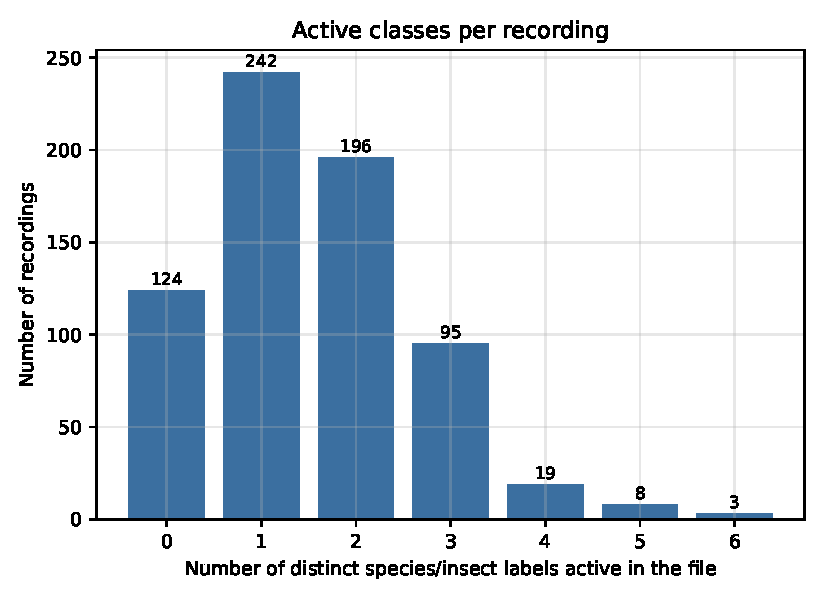
\includegraphics[width=0.7\textwidth]{figures/08_active_classes_per_file.pdf}
\caption{Active (distinct) classes per recording --- right-skewed,
mode-at-1, matching Morfi et al.\ Fig.~3.}
\label{fig:08}
\end{figure}

\subsubsection{Overlap / co-occurrence --- a form of structural label noise}
\label{sec:A55}

A sweep-line over every file's tagged intervals gives, second-by-second, how
many tags are simultaneously active --- reproducing Morfi et al.\ Fig.~5
essentially exactly:

\begin{table}[h]
\centering
\caption{Simultaneity of active tags (sweep-line, this analysis vs.\ Morfi et al.).}
\begin{tabular}{l c c}
\toprule
simultaneously active tags & this analysis & Morfi et al., Fig.~5 \\
\midrule
0 & 66.32\% & 66.3\% \\
1 & 28.09\% & 28.1\% \\
2 & 5.24\%  & 5.2\%  \\
3 & 0.36\%  & 0.4\%  \\
\bottomrule
\end{tabular}
\end{table}

\begin{figure}[h]
\centering
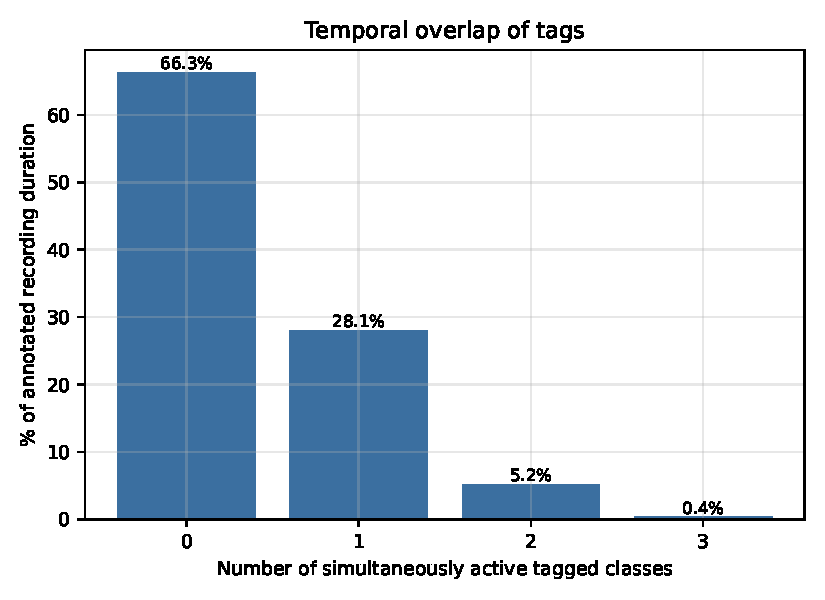
\includegraphics[width=0.75\textwidth]{figures/09_simultaneity.pdf}
\caption{Simultaneity histogram, sweep-line over all annotated intervals.}
\label{fig:09}
\end{figure}

At the individual-event level: \textbf{27.4\%} of the 5{,}775 tagged events
overlap in time with at least one other tagged event; \textbf{24.0\%} with a
\emph{different-label} tag --- corroborating the paper's ``over 20\% of
tagged sounds overlap with sounds of other species'' from an independent
computation path. At the label level, \textbf{81 of 89 distinct labels
(91\%)} have been recorded overlapping with at least one other label
somewhere in the corpus, driven disproportionately by long-duration insect
stridulation songs acting as a near-continuous background.

\begin{figure}[h]
\centering
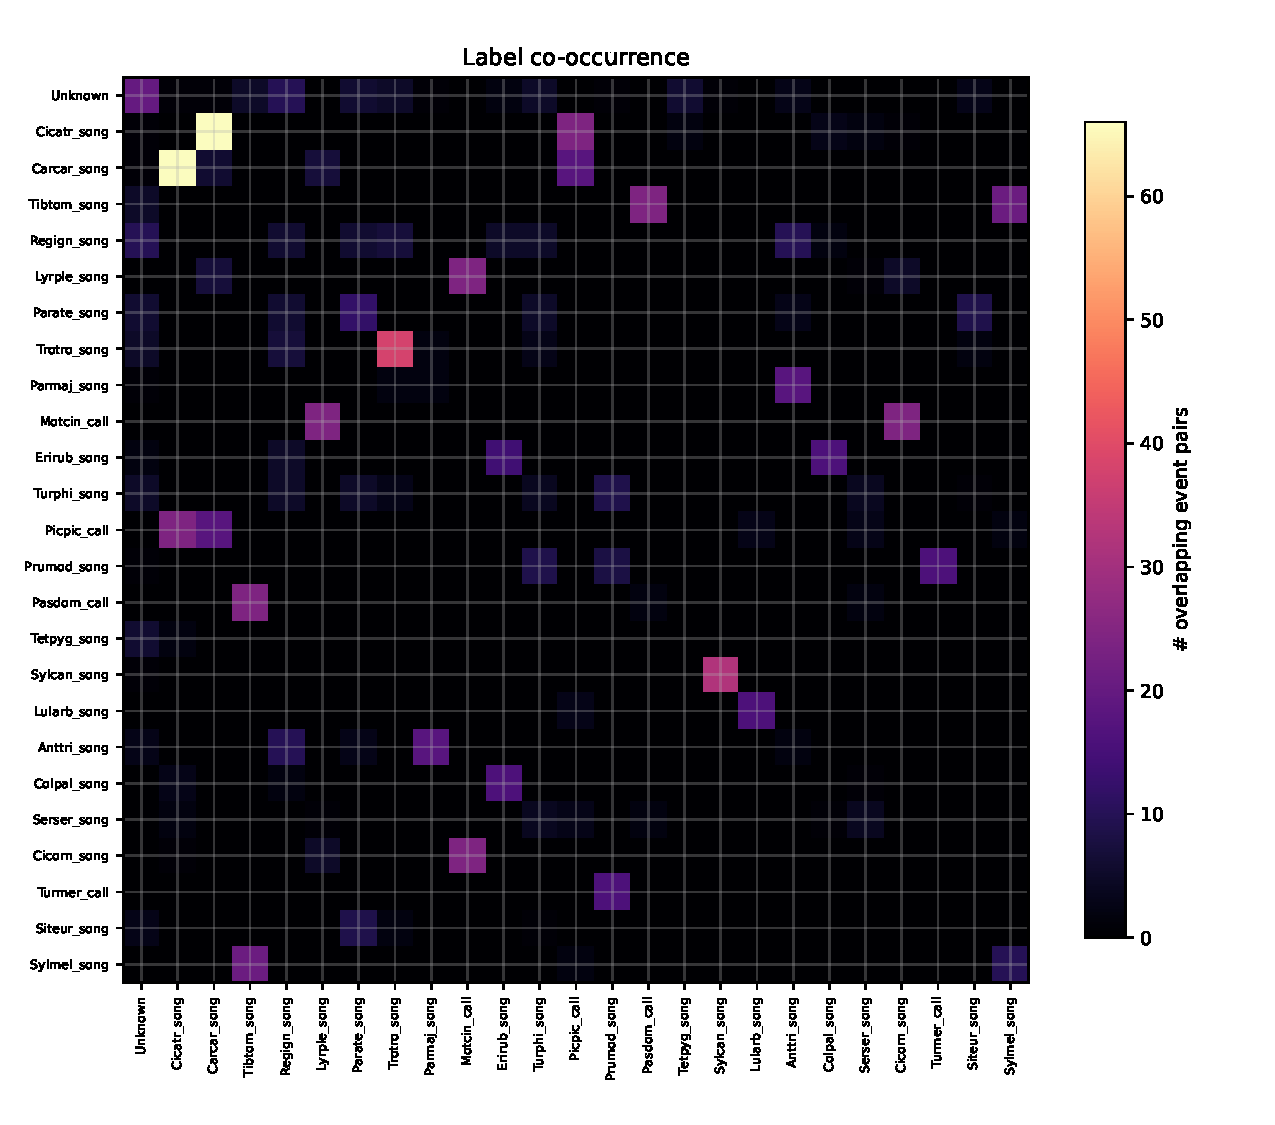
\includegraphics[width=0.75\textwidth]{figures/10_cooccurrence_heatmap.pdf}
\caption{Label-pair co-occurrence heatmap. Strongest pairs are dominated by
insect songs (e.g.\ \texttt{Carcar\_song}$\leftrightarrow$\texttt{Cicatr\_song},
66 overlapping instances).}
\label{fig:10}
\end{figure}

\begin{figure}[h]
\centering
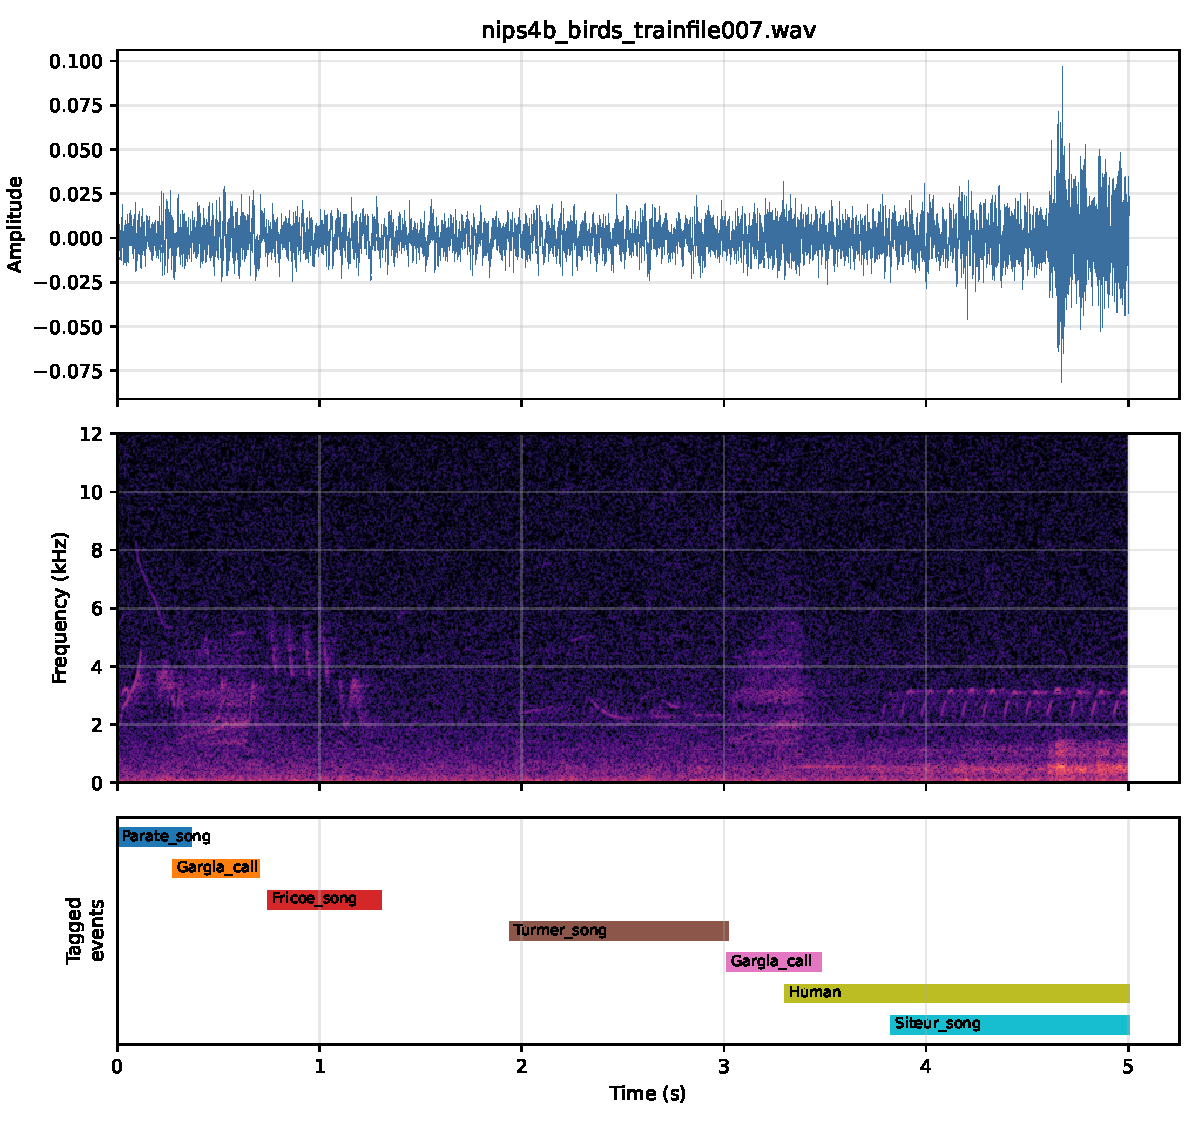
\includegraphics[width=0.85\textwidth]{figures/15_multi_tag_example_trainfile007.pdf}
\caption{\texttt{nips4b\_birds\_trainfile007.wav}: 7 tagged events, 5
species, plus an overlapping \texttt{Human} tag --- waveform, spectrogram,
and tag timeline on a shared time axis.}
\label{fig:15}
\end{figure}

This matters statistically because every overlapping window is a case where
the \emph{acoustic content} the model sees during training is a mixture of
two sources, but the \emph{label} names only one of them --- a structural,
non-random source of label noise that no amount of extra training data
removes.

\subsubsection{Summary --- ``is it normally distributed?''}

\begin{table}[h]
\centering
\begin{tabularx}{\textwidth}{l c Y}
\toprule
Feature family & Practically normal? & Actual shape \\
\midrule
File/event duration & No --- censored mixture (files) / lognormal (events) & bimodal-ish ceiling+tail (files); lognormal, median $\ll$ mean (events) \\
Amplitude (RMS, crest factor) & No & Lognormal, heavy right skew, extreme-outlier-driven kurtosis \\
Spectral centroid/bandwidth & Approximately (best fit only marginally beats Normal) & Weibull $\approx$ Normal --- an averaged quantity, pulled toward Gaussian by construction \\
Class frequency (target variable) & No & Zipf-like, moderate long tail, $31.3\times$ max/min \\
\bottomrule
\end{tabularx}
\end{table}

\subsection{Evaluation metrics --- formal definitions}
\label{sec:A6}

\texttt{evaluate\_metrics.py} (this repository's reconstruction of the
paper's Table~1 methodology) computes, per class scheme, from
$y_{\text{true}}\in\{1,\dots,C\}^N$, $y_{\text{pred}}$, and score matrix
$S\in\mathbb{R}^{N\times C}$:

\[
\text{Accuracy} = \frac{1}{N}\sum_{i=1}^N \mathbb{1}[y_i=\hat y_i]
\]
\[
\text{Precision}_{\text{weighted}} = \sum_{c=1}^C \frac{n_c}{N}\cdot\frac{TP_c}{TP_c+FP_c},
\qquad
\text{Recall}_{\text{weighted}} = \sum_{c=1}^C \frac{n_c}{N}\cdot\frac{TP_c}{TP_c+FN_c}
\]
\[
\text{ROC-AUC}_{\text{weighted, OvR}} = \sum_{c=1}^C \frac{n_c}{N}\cdot\text{AUC}\big(\mathbb{1}[y=c],\ S_{:,c}\big)
\]
\[
\text{Top-}k = \frac{1}{N}\sum_{i=1}^N \mathbb{1}\Big[y_i \in \operatorname{argtop}_k\big(S_{i,:}\big)\Big]
\]

\textbf{A provable identity}, confirmed in this codebase and in the paper's
Table~1: for single-label multiclass classification, weighted recall is
\emph{algebraically identical} to accuracy:
\[
\text{Recall}_{\text{weighted}} = \sum_{c=1}^C \frac{n_c}{N}\cdot\frac{TP_c}{n_c}
= \frac{1}{N}\sum_{c=1}^C TP_c
= \frac{\text{total correct}}{N} = \text{Accuracy},
\]
since $FN_c$'s denominator $TP_c+FN_c$ is exactly $n_c$ (every true instance
of class $c$ is either a $TP_c$ or an $FN_c$; there is no notion of a
class-$c$ instance being ``missed entirely'' the way there would be in
detection). This is why the paper's Table~1 shows Recall $=$ Accuracy on
every row --- a mathematical consequence of the metric choice for this task
shape, not a coincidence.

Sentence/file-level scores feeding these metrics come from summing per-frame
log-probabilities across a dense sliding window over the \emph{whole} test
file and re-softmaxing (Section~\ref{sec:C2}) --- \textbf{not} the paper's
own stated methodology of ``mean posterior probability over each tagged
call,'' which would restrict scoring to the event's own span (Section~\ref{sec:A7}).

\subsection{Scope, limitations, and critique}
\label{sec:A7}

\textbf{What the task legitimately achieves.} It is a clean, well-posed,
closed-set multiclass classification problem with a sensible metric suite
(accuracy/AUC as headline numbers, top-$k$ as a softer measure appropriate
given the moderate class count and imbalance, weighted averaging so minority
classes aren't invisible to precision/recall). The raw-waveform-plus-constrained-filterbank
design is well-motivated by the EDA in Section~\ref{sec:A53}: call durations
are genuinely too short and too heavy-tailed for a speech-scale analysis
window, and this is demonstrated quantitatively, not asserted. The paper is
honest about its own ceiling --- no architecture it tried (SincNet,
ResNet50, VGG16, DenseNet121) exceeds 80\% accuracy, and it states this
plainly as a sign of task difficulty.

\textbf{Where the problem formulation is weaker than it first appears:}

\begin{enumerate}
\item \textbf{The evaluation task is not what it's framed as.} The paper
  frames Table~1 as ``how well does the model classify a \emph{tagged
  call},'' but the scoring code evaluates over the \textbf{entire
  recording}, of which the tagged event occupies as little as 1.1--7.3\%
  (measured on a 5-row sample against files on disk). A model that mostly
  learns ``what does this \emph{recording} sound like'' rather than ``what
  does this \emph{call} sound like'' would still score well under this
  metric.

\item \textbf{Train/test leakage at the unit-of-splitting level.} The split
  is drawn over individual \emph{tags}, not source \emph{recordings}: of 429
  unique files in the bird-classes test list, 414 (96.5\%) also contribute a
  \emph{different} tagged row to the training set. The paper's own
  Discussion names this exact effect (``drawing training and test sets from
  the same data pool is known to simplify the task''), so this is a known,
  acknowledged limitation --- but Table~1's numbers should be read as an
  upper bound on genuinely-novel-recording performance, not an unbiased
  estimate of it.

\item \textbf{Label noise is structural, not just annotator error.}
  24--27\% of tagged events overlap another tag (Section~\ref{sec:A55}). A
  single-label classifier trained on a window that genuinely contains two
  species' calls is, by construction, trained against an incomplete label
  for a non-trivial fraction of its training signal.

\item \textbf{A non-reproducible target variable.} Because
  \texttt{generate\_mod\_file\_lists.py} calls \texttt{train\_test\_split}
  with no \texttt{random\_state}, both the train/test partition \emph{and}
  the integer$\to$class label mapping change on every regeneration.
  Re-scoring an old checkpoint against a freshly regenerated list gives
  near-random accuracy, not because the checkpoint is bad, but because class
  index 7 under the old split is a different species under the new one --- a
  genuine reproducibility gap.

\item \textbf{Single annotator, single pass.} Every duration/overlap
  statistic here (and every label in the dataset) reflects one person's
  judgment calls about where a call starts and ends; the paper itself flags
  inconsistency across files. There is no second annotator's labels to
  separate genuine acoustic variability from annotation-style variability.

\item \textbf{Verified discrepancies between the papers' text and the
  released data:} bit depth (paper: 32-bit; files: 16-bit PCM), insect
  species count (paper: 7; files: 9), ``61 bird species'' (actually 61
  organisms across all taxa, 51 of which are birds), empty-annotation-file
  count (paper: $\sim$100; files: 105), test-set duration (paper: ``nearly
  two hours''; measured: 69.5~min).
\end{enumerate}

% ======================================================================
\section{Part B --- Methodological Justification}
% ======================================================================

\subsection{Why raw waveform, why a constrained first layer}
\label{sec:B1}

The methodological chain, grounded in Part A's EDA:

\begin{enumerate}[nosep]
\item Conventional bioacoustic pipelines hand-design a spectral
  representation (MFCC/Mel) before classification --- importing frame
  lengths and frequency-warping assumptions tuned for human speech.
\item Part A's EDA shows tagged bird-call durations are lognormally
  distributed with a $\sim$90~ms median (Section~\ref{sec:A53}) --- an order
  of magnitude shorter than the 200~ms frame conventional in speech
  processing.
\item Therefore the authors (a)~shrink the frame drastically (200~ms
  $\to$ 10--18~ms) and (b)~replace the hand-designed spectral front-end with
  a \textbf{learned but DSP-constrained} filterbank (\texttt{SincConv}) that
  discovers which frequency bands matter for \emph{this} task.
\end{enumerate}

The mathematical case for the constraint: an ordinary learned 1-D
convolutional filter of length $L$ has $L$ free parameters; constraining it
to be a symmetric band-pass filter parameterised only by its cutoffs
$(f_l,f_h)$ reduces this to 2 parameters per filter:
\[
g[n; f_l, f_h] = 2f_h\,\operatorname{sinc}(2\pi f_h n) - 2f_l\,\operatorname{sinc}(2\pi f_l n),
\qquad \operatorname{sinc}(x)=\frac{\sin x}{x},
\]
windowed by a Hamming function $w[n]=0.54-0.46\cos(2\pi n/L)$ to make the
theoretically-infinite sinc implementable. This rests on the standard DSP
identity that an ideal band-pass filter's impulse response is the
difference of two sinc-shaped low-pass responses (rectangular frequency
response $\Leftrightarrow$ sinc time response, via the inverse Fourier
transform); the paper's contribution is making $(f_l,f_h)$
\textbf{learnable} via backpropagation rather than fixed by a DSP designer.

\begin{figure}[h]
\centering
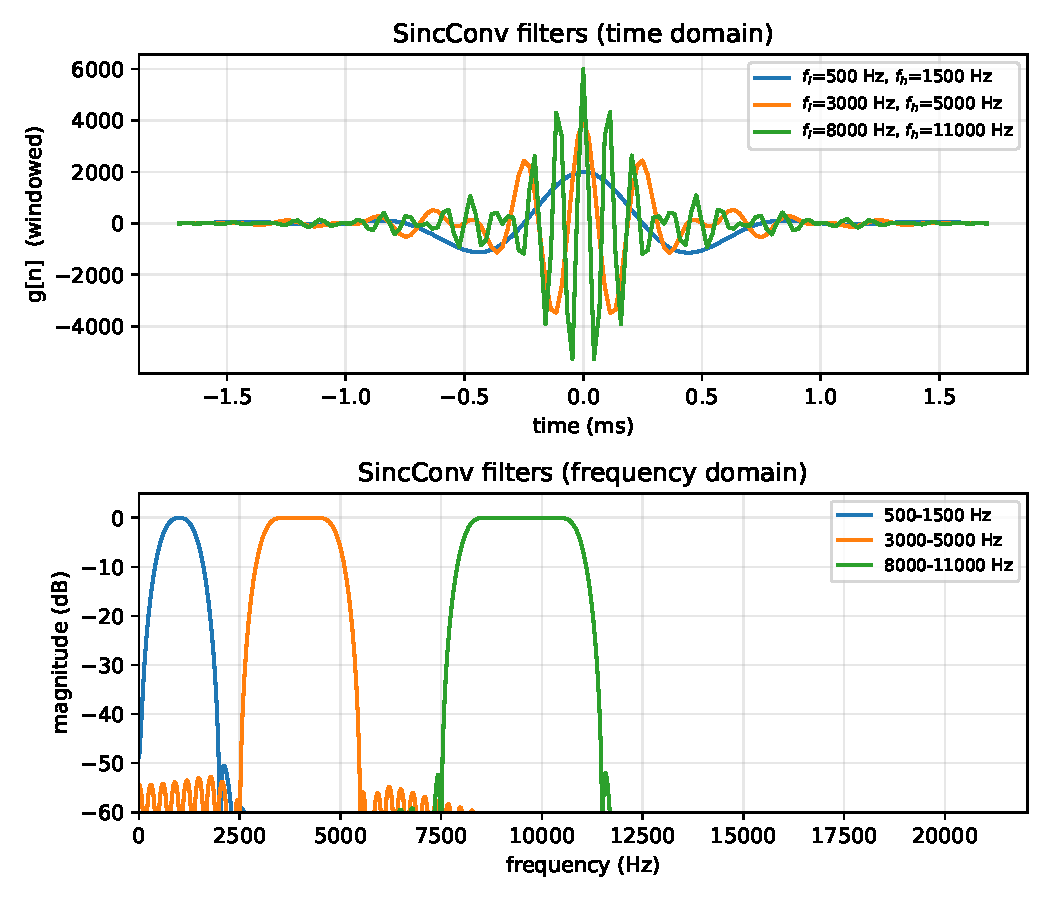
\includegraphics[width=0.85\textwidth]{figures/16_sincconv_filter_response.pdf}
\caption{Illustrative SincConv band-pass filters (own computation from the
closed-form definition, $L=151$, three example $(f_l,f_h)$ pairs). Top: the
time-domain, Hamming-windowed filter $g[n]$. Bottom: its magnitude frequency
response, approximating a rectangular passband between $f_l$ and $f_h$.}
\label{fig:16}
\end{figure}

For the enhanced architecture's 220 filters of length 151, this is
$220\times151=33{,}220$ unconstrained parameters collapsed to
$220\times2=440$ --- a \textbf{75.5$\times$ reduction} in the first layer's
degrees of freedom, precisely the kind of inductive bias that matters on a
dataset this small (3,957--4,110 training tags).

\placeholderfig{a scatter plot of each Sinc filter's \emph{learned} cutoff
pair $(f_l,f_h)$ after training, plotted against its Mel-scale
\emph{initial} cutoff pair --- the diagnostic the paper itself reports to
show how little the filters move from initialization. Requires a trained
model checkpoint's actual filter weights; no such checkpoint with verified
provenance exists in this reproduction session (Section~\ref{sec:A7}, item
4), so this cannot be fabricated from data on hand.}{Placeholder --- learned
vs.\ Mel-initialised Sinc filter cutoffs (would require a trained,
provenance-verified checkpoint).}

\textbf{A caveat the paper itself raises:} in the efficient
(\texttt{SincConv\_fast}) implementation, the learned filters move
relatively little from their Mel-scale initialisation --- the front-end
behaves, empirically, closer to ``a carefully chosen fixed filterbank plus
light task-specific fine-tuning'' than ``fully free filter discovery.''
Since Mel-scale spacing is itself a human-hearing prior, this partially
reintroduces, via initialisation, exactly the kind of anthropocentric
assumption the raw-waveform approach was chosen to avoid.

\subsection{The end-to-end workflow}
\label{sec:B2}

\begin{figure}[h]
\centering
\resizebox{\textwidth}{!}{%
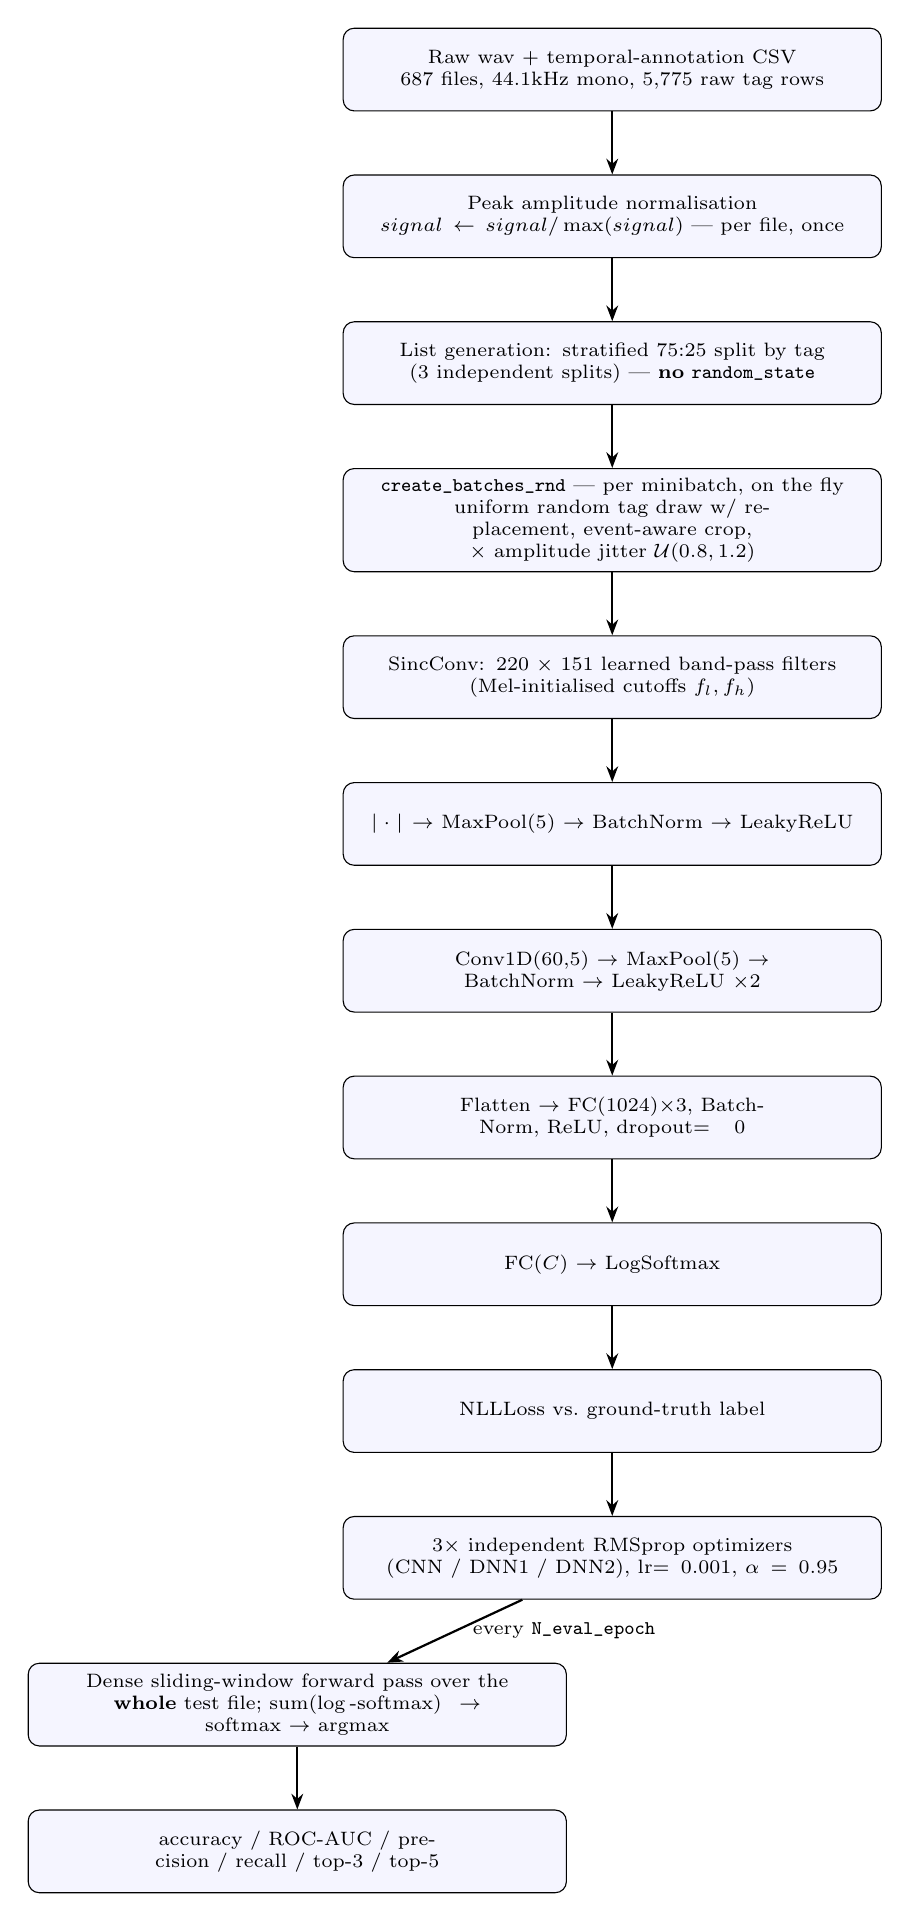
\begin{tikzpicture}[
  node distance=8mm and 8mm,
  box/.style={rectangle, draw, rounded corners, fill=blue!4, align=center,
    text width=6.6cm, minimum height=1.05cm, font=\scriptsize},
  arr/.style={-{Stealth[length=2mm]}, thick}
]
\node[box] (a) {Raw wav + temporal-annotation CSV\\687 files, 44.1kHz mono, 5{,}775 raw tag rows};
\node[box, below=of a] (b) {Peak amplitude normalisation\\$signal \gets signal/\max(signal)$ --- per file, once};
\node[box, below=of b] (c) {List generation: stratified 75:25 split by tag\\(3 independent splits) --- \textbf{no} \texttt{random\_state}};
\node[box, below=of c] (d) {\texttt{create\_batches\_rnd} --- per minibatch, on the fly\\uniform random tag draw w/ replacement, event-aware crop,\\$\times$ amplitude jitter $\mathcal{U}(0.8,1.2)$};
\node[box, below=of d] (e) {SincConv: $220\times151$ learned band-pass filters\\(Mel-initialised cutoffs $f_l,f_h$)};
\node[box, below=of e] (f) {$|\cdot| \to$ MaxPool(5) $\to$ BatchNorm $\to$ LeakyReLU};
\node[box, below=of f] (g) {Conv1D(60,5) $\to$ MaxPool(5) $\to$ BatchNorm $\to$ LeakyReLU $\times 2$};
\node[box, below=of g] (h) {Flatten $\to$ FC(1024)$\times$3, BatchNorm, ReLU, dropout$=0$};
\node[box, below=of h] (i) {FC($C$) $\to$ LogSoftmax};
\node[box, below=of i] (j) {NLLLoss vs.\ ground-truth label};
\node[box, below=of j] (k) {3$\times$ independent RMSprop optimizers\\(CNN / DNN1 / DNN2), lr$=0.001$, $\alpha=0.95$};
\node[box, below=of k, xshift=-4cm] (l) {Dense sliding-window forward pass over the\\\textbf{whole} test file; $\operatorname{sum}(\log\text{-softmax}) \to$ softmax $\to$ argmax};
\node[box, below=of l] (m) {accuracy / ROC-AUC / precision / recall / top-3 / top-5};

\draw[arr] (a)--(b); \draw[arr] (b)--(c); \draw[arr] (c)--(d);
\draw[arr] (d)--(e); \draw[arr] (e)--(f); \draw[arr] (f)--(g);
\draw[arr] (g)--(h); \draw[arr] (h)--(i); \draw[arr] (i)--(j);
\draw[arr] (j)--(k);
\draw[arr] (k) -- node[right, font=\scriptsize, xshift=1mm]{every \texttt{N\_eval\_epoch}} (l);
\draw[arr] (l)--(m);
\end{tikzpicture}}
\caption{End-to-end training/evaluation workflow, as actually executed by
\texttt{call\_id.py} and \texttt{evaluate\_metrics.py}.}
\label{fig:workflow}
\end{figure}

\subsection{Microscopic, layer-by-layer justification}
\label{sec:B3}

\subsubsection{Peak-normalise: per-file amplitude ``scaling''}
\label{sec:B31}

\begin{lstlisting}[language=Python]
signal = signal.astype(np.float64)
signal = signal / np.abs(np.max(signal))
\end{lstlisting}

\textbf{Yes, this is a scaling step}, and it is the \emph{only} one in the
entire pipeline. Its purpose is legitimate: field recordings vary enormously
in absolute level depending on the vocalising animal's distance and the
recorder's gain setting, and bringing every file to a common peak amplitude
removes that nuisance variable before the model sees the signal.
\textbf{Mathematically, however, it is a fragile choice} given Part A's
finding that RMS energy and crest factor are lognormally distributed with
extreme kurtosis (Table~\ref{tab:waveform-stats}): normalising by the single
most extreme \emph{signed} sample (\texttt{np.max}, not
\texttt{np.max(np.abs(...))}) makes the scaling factor for an entire file a
statistic driven by one outlier sample --- exactly the situation the
\texttt{trainfile439}-style impulsive outlier (Figure~\ref{fig:14})
demonstrates is common in this corpus. A theoretically more robust choice
--- scaling by RMS energy, or a log-compressive transform --- would be more
consistent with the \emph{measured} shape of the amplitude distribution.
(The sign bug specifically --- dividing by $\max(\text{signal})$ rather than
$\max(|\text{signal}|)$, which can push the ``normalised'' signal past
$\pm1.0$ whenever the largest excursion is negative --- is a genuine
implementation error, affecting 47/200 spot-checked files up to
$1.38\times$ overshoot, and is left as-is since it is the authors' own
released preprocessing.)

\subsubsection{Event-aware windowing: the dataset's own shape forcing a code branch}
\label{sec:B32}

\texttt{create\_batches\_rnd} computes, per drawn tag,
$t_{\min}=\lfloor \text{start}\cdot f_s\rfloor$,
$t_{\max}=t_{\min}+\lfloor \text{length}\cdot f_s\rfloor$, then:
\[
\text{signal\_start} \sim
\begin{cases}
\mathcal{U}\{t_{\min},\, t_{\max}-w\} & \text{if } t_{\max}-t_{\min} > w
\quad(\text{window wholly inside event}) \\[4pt]
\mathcal{U}\{\max(0, t_{\max}-w),\, \min(t_{\min}, L-w)\} & \text{otherwise}
\quad(\text{window contains the whole event})
\end{cases}
\]
where $L$ is the file length in samples. This two-branch logic exists
\emph{because} of the fact established in Section~\ref{sec:A53}: the
lognormal duration distribution has enough right-tail mass that most events
are longer than the 16--18~ms window (first branch: crop inside), but a
measurable minority (14/5{,}775) are shorter and must instead be padded with
surrounding context (second branch). \textbf{This is functionally a
data-augmentation step as well as a windowing step}: because the crop
position is redrawn uniformly at random on every minibatch draw, the same
tagged event is seen at a different temporal offset nearly every time it's
sampled --- on top of which a \textbf{separate}, explicit amplitude-jitter
augmentation is applied:
\[
x'_i = a_i \cdot x_i, \qquad a_i \sim \mathcal{U}(0.8, 1.2) \quad
(\text{\texttt{fact\_amp}}=0.2,\ \text{hard-coded in \texttt{call\_id.py}}).
\]
This is well-justified: the model should not learn to rely on absolute
recording level. Note the enhanced-model configs expose no \texttt{fact\_amp}
field at all (it is read from the call site's literal \texttt{0.2}, not the
\texttt{[optimization]} section), so despite the paper discussing disabling
this augmentation for the enhanced experiments, that setting is not
reachable from the tracked config files.

\subsubsection{SincConv: the constrained first layer}
\label{sec:B33}

Already derived mathematically in Section~\ref{sec:B1}. Two further
justification points:

\begin{itemize}
\item \textbf{Mel initialisation.} Cutoffs are initialised via
  $m = 2595\log_{10}(1+f/700)$ (Hz$\to$Mel) so initial filter spacing is
  denser at low frequencies, matching where more acoustically relevant
  structure typically lives --- a reasonable starting-point prior, even
  though (per Section~\ref{sec:B1}'s caveat) the filters do not move very
  far from it during training.
\item \textbf{Nyquist bound.} With $f_s=44{,}100$~Hz, the maximum
  representable frequency is $f_s/2=22{,}050$~Hz --- the implementation
  clips learned $f_h$ to this bound, and it is the direct reason the
  44.1~kHz sampling rate matters methodologically: a 16~kHz speech-derived
  sampling rate (Nyquist 8~kHz) would make a large fraction of the spectral
  content available to this filterbank simply inaccessible, regardless of
  architecture.
\end{itemize}

\subsubsection{Normalisation layers: LayerNorm (default) vs.\ BatchNorm (enhanced) --- stated explicitly}
\label{sec:B34}

Reading the tracked config files directly:

\begin{table}[h]
\centering
\begin{tabularx}{\textwidth}{l Y Y}
\toprule
 & default / Part I (\texttt{cfg/*.cfg}) & enhanced / Part II (\texttt{mod\_cfg/*.cfg}) \\
\midrule
CNN layers & \texttt{cnn\_use\_laynorm=True,True,True}; \texttt{cnn\_use\_batchnorm=False,False,False} & \texttt{cnn\_use\_laynorm=False,False,False}; \textbf{\texttt{cnn\_use\_batchnorm=True,True,True}} \\
FC layers  & \texttt{fc\_use\_batchnorm=True,True,True} (both configs) & \texttt{fc\_use\_batchnorm=True,True,True} \\
\bottomrule
\end{tabularx}
\end{table}

\textbf{Yes --- batch normalisation is used}, in both configurations' FC
stack, and additionally in the CNN stack for the enhanced models
specifically (replacing LayerNorm there). Justification:
\[
\hat x = \frac{x-\mu_B}{\sqrt{\sigma_B^2+\epsilon}}, \qquad y=\gamma\hat x+\beta .
\]
BatchNorm normalises each channel's activations using the current
minibatch's mean/variance, which (a)~reduces internal covariate shift
layer-to-layer, letting the network tolerate a higher learning rate without
diverging, and (b)~provides a mild regularising effect from batch-to-batch
statistic variability --- genuinely useful given the FC stack here has
\textbf{zero dropout} (Section~\ref{sec:B38}). It requires a reasonably
large, representative batch (used here at \texttt{batch\_size=128}). LayerNorm,
by contrast, normalises across the \emph{feature} dimension within a single
example --- independent of batch composition, more robust when batch
statistics might be noisy. The switch from LayerNorm (default CNN) to
BatchNorm (enhanced CNN) is consistent with a standard modern-deep-learning
heuristic rather than being traceable to any bioacoustic-specific argument
in the paper's text --- likely an empirical/engineering choice from the
described hyperparameter sweep, not a domain-motivated one.

\subsubsection{Activation functions}

CNN layers use \texttt{leaky\_relu} in both configs; FC layers use
\texttt{leaky\_relu} (default) or \texttt{relu} (enhanced).
\[
\operatorname{LeakyReLU}(x)=\begin{cases}x & x\ge0\\ 0.01x & x<0\end{cases}
\]
avoids the ``dying ReLU'' failure mode by keeping a small non-zero gradient
in the negative regime --- a reasonable default for a from-scratch CNN stack
with no pretrained initialisation to lean on. Plain \texttt{relu} in the
enhanced FC stack is defensible given BatchNorm precedes it in both configs,
mitigating the risk of large sustained negative pre-activations killing
units.

\subsubsection{Pooling}

Default: \texttt{MaxPool(3)} $\times 3$; enhanced: \texttt{MaxPool(5)}
$\times 3$. Max pooling over the sinc-filtered signal builds local
time-shift invariance and reduces sequence length before the next
convolution --- appropriate since the exact sample-level phase of a bird
call's acoustic energy within its window is not discriminative; what
matters is which frequency bands are active, not their precise alignment to
a sample index. The enhanced model's shorter input window (705 vs.\ 441
samples) and shorter first-layer filter (151 vs.\ 251) are compensated by a
larger pool factor (5 vs.\ 3) to still reach a comparably small flattened
dimensionality (180 vs.\ 300) feeding the FC stack.

\subsubsection{Ordinary Conv1D layers}

Two \texttt{Conv1D(60, kernel=5)} layers follow SincConv in both configs,
operating on the already frequency-decomposed 220- (or 80-) channel
representation, learning combinations across channels and short-range
temporal patterns. This is architecturally standard and not claimed as
novel; its role is to let Level-2 (local structure) abstraction happen on
top of Level-1 (frequency decomposition) before Level-3 (FC, species-level
combination).

\subsubsection{Fully-connected stack, and zero dropout}
\label{sec:B38}

\texttt{fc\_lay=2048,2048,2048} (default) or \texttt{1024,1024,1024}
(enhanced), \textbf{with \texttt{cnn\_drop}, \texttt{fc\_drop}, and
\texttt{class\_drop} all set to \texttt{0.0} in every single tracked config
file}, default and enhanced alike. This is a direct, explicit-from-the-config
finding: \textbf{no dropout is used anywhere in this pipeline as currently
configured.} Given (a)~a training pool of only 3,957--4,110 tags feeding up
to 87 output classes, (b)~wide FC layers, and (c)~the class-imbalance
profile of Section~\ref{sec:A54}, this is a textbook overfitting setup ---
independently corroborated by the actually-trained checkpoints in this
reproduction: all three prior runs show training error falling to
0.14--0.21 while test error plateaus around 0.60, the canonical signature of
a model with far more capacity than regularisation. The paper's text does
mention dropout as a \emph{swept} hyperparameter, so it is plausible the
authors' own best Table-1 models used non-zero values recorded only in an
inaccessible supplementary document --- but the configs that actually ship
and run in this checkout use zero throughout, methodologically the weakest
single link in the regularisation story as implemented.

\subsubsection{Output layer: config says ``softmax,'' code does \texttt{LogSoftmax} + \texttt{NLLLoss}}

\texttt{class\_act=softmax} in every config, but the actual model
implementation applies \texttt{LogSoftmax} at the output and pairs it with
\texttt{nn.NLLLoss()}. This is not a discrepancy in practice --- for target
$y$ and log-probabilities $\log\hat p$,
\[
\text{NLLLoss}(\log\hat p, y) = -\log \hat p_y = -\log\frac{e^{z_y}}{\sum_c e^{z_c}}
\]
is \textbf{exactly} standard categorical cross-entropy
$-\sum_c \mathbb{1}[c=y]\log \hat p_c$ evaluated on a one-hot target ---
\texttt{LogSoftmax} + \texttt{NLLLoss} is mathematically identical to
\texttt{Softmax} + categorical cross-entropy, computed in a numerically more
stable order. The config field name is simply a label for ``use a
categorical classification head here,'' not a literal claim about which
activation tensor is materialised.

\subsubsection{Optimizer: three independent RMSprop instances}
\label{sec:B310}

\begin{lstlisting}[language=Python]
optimizer_CNN  = optim.RMSprop(CNN_net.parameters(),  lr=lr, alpha=0.95, eps=1e-8)
optimizer_DNN1 = optim.RMSprop(DNN1_net.parameters(), lr=lr, alpha=0.95, eps=1e-8)
optimizer_DNN2 = optim.RMSprop(DNN2_net.parameters(), lr=lr, alpha=0.95, eps=1e-8)
\end{lstlisting}

RMSprop's update rule, per parameter $\theta$ with gradient $g_t$:
\[
v_t = \alpha v_{t-1} + (1-\alpha) g_t^2, \qquad
\theta_t = \theta_{t-1} - \frac{\eta}{\sqrt{v_t}+\epsilon}\, g_t
\]
with $\alpha=0.95$, $\eta=0.001$, $\epsilon=10^{-8}$. \textbf{Why RMSprop
over plain SGD or Adam here is a reasonable choice:} the network's parameter
groups have genuinely different natural scales --- the SincConv layer's
$f_l,f_h$ live on a Hz scale (0--22,050), while the FC layers' weights are
on the usual small-magnitude scale --- and RMSprop's per-parameter adaptive
step size is specifically designed to handle this kind of scale
heterogeneity without requiring careful per-group learning-rate tuning, as
plain SGD would. Using \textbf{three separate optimizer instances} rather
than one optimizer over all parameters is functionally equivalent to one
optimizer with three parameter groups (each maintains its own $v_t$
per-parameter regardless) --- a code-organisation choice, not a distinct
optimisation strategy.

There is \textbf{no learning-rate schedule} anywhere in the training
script --- $\eta$ is held at a constant 0.001 for all 200--400 epochs.
Given RMSprop's adaptive per-parameter scaling already provides some
automatic step-size moderation near convergence, a fixed global $\eta$ is a
defensible simplification, though a decay schedule is a standard, low-risk
addition (Section~\ref{sec:C4}).

\subsubsection{Hyperparameters and epoch semantics}

\begin{table}[h]
\centering
\begin{tabular}{l c c}
\toprule
 & default & enhanced \\
\midrule
\texttt{lr} & 0.001 & 0.001 \\
\texttt{batch\_size} & 128 & 128 \\
\texttt{N\_epochs} & 200 & 400 \\
\texttt{N\_batches} & 800 & 80 \\
examples seen per ``epoch'' & $800\times128=102{,}400$ & $80\times128=10{,}240$ \\
total gradient steps, full run & $200\times800=160{,}000$ & $400\times80=32{,}000$ \\
\bottomrule
\end{tabular}
\end{table}

Because sampling is \textbf{with replacement, uniformly over tags, on the
fly}, ``epoch'' here is purely a bookkeeping unit for when
validation/checkpointing runs (\texttt{N\_eval\_epoch=8}) --- it does
\textbf{not} mean ``one pass through the training set.'' The enhanced
config's nominal 400 epochs is, in total gradient steps, actually
\textbf{5$\times$ fewer} than the default's nominal 200 epochs
(32{,}000 vs.\ 160{,}000) --- comparing ``epoch count'' across these two
configs without multiplying through by \texttt{N\_batches} would be a
direct methodological error.

\subsection{Data-splitting strategy --- assessed}
\label{sec:B4}

\texttt{train\_test\_split(..., test\_size=0.25, stratify=<class column>)},
called \textbf{three independent times} with \textbf{no
\texttt{random\_state}}. Stratification by class is the right call for an
imbalanced target (Section~\ref{sec:A54}) --- it guarantees each class's
train/test proportion tracks its overall frequency. But the \textbf{unit
being split is the tag, not the source recording} --- the split does not
know or care that many tags share a parent file --- which is what produces
the measured 96.5\% file-overlap leakage (Section~\ref{sec:A7}, item 2).
Combined with the missing \texttt{random\_state}, every re-run of list
generation invalidates every existing checkpoint's label mapping.

\subsection{Model-selection strategy --- assessed}
\label{sec:B5}

The paper describes, for Part~I, five independent training runs per class
scheme under different random splits; for Part~II, ``the best performing
models reported in the results use combinations of the best parameter
values'' --- an informal manual/grid search over filter counts, filter
lengths, normalisation type, dropout, and \texttt{fact\_amp}. This is
\textbf{best-of-$N$ selection against the same held-out test set that is
then reported as the final number} --- there is no separate validation
split distinct from the reported test set visible in any config here
(\texttt{tr\_lst}/\texttt{te\_lst} only). Statistically, repeatedly
evaluating different configurations against one fixed held-out set and
reporting the winner's score on that same set is a well-known source of
\textbf{optimistic bias}.

\subsection{Scorecard: what's mathematically sound vs.\ questionable}

\begin{table}[h]
\centering
\small
\begin{tabularx}{\textwidth}{Y Y}
\toprule
Component & Assessment \\
\midrule
SincConv parameterisation ($75.5\times$ parameter reduction) & Sound --- standard DSP identity, appropriate inductive bias for a small dataset \\
Mel initialisation of filter cutoffs & Reasonable prior; caveat that filters move little from it in practice \\
Peak amplitude normalisation & Legitimate purpose, but statistically fragile given measured lognormal/kurtotic amplitude distribution; implementation also has a signed-max bug \\
On-the-fly random windowing + amplitude jitter & Sound as augmentation; directly motivated by the measured event-duration distribution \\
BatchNorm (enhanced) / LayerNorm (default) & Both defensible; the specific choice reads as empirical, not domain-derived \\
LeakyReLU / ReLU & Standard, appropriate given BatchNorm precedes ReLU in the FC stack \\
Zero dropout across every tracked config & Weakest link --- directly consistent with the measured overfitting \\
LogSoftmax + NLLLoss (labelled ``softmax'' in config) & Mathematically correct ($=$ standard cross-entropy); naming is misleading, not a defect \\
3$\times$ RMSprop, constant LR, no schedule & Reasonable given heterogeneous parameter scales; no schedule is a simplification \\
Stratified but tag-level, unseeded 75:25 split & Correct on the imbalance axis; unsound on the leakage and reproducibility axes \\
Best-of-N model selection against the reported test set & Common practice, but a known source of optimistic bias \\
Whole-file dense evaluation, sum-then-argmax & Mathematically well-defined, but scores a different task than the paper's own stated methodology \\
\bottomrule
\end{tabularx}
\end{table}

% ======================================================================
\section{Part C --- Data Pipeline Analysis}
% ======================================================================

\subsection{Pipeline diagram}
\label{sec:C1}

Two structurally independent pipelines share the same raw inputs and never
converge; only the right-hand branch is what every enhanced config (and
therefore every checkpoint) actually consumes.

\begin{figure}[h]
\centering
\resizebox{\textwidth}{!}{%
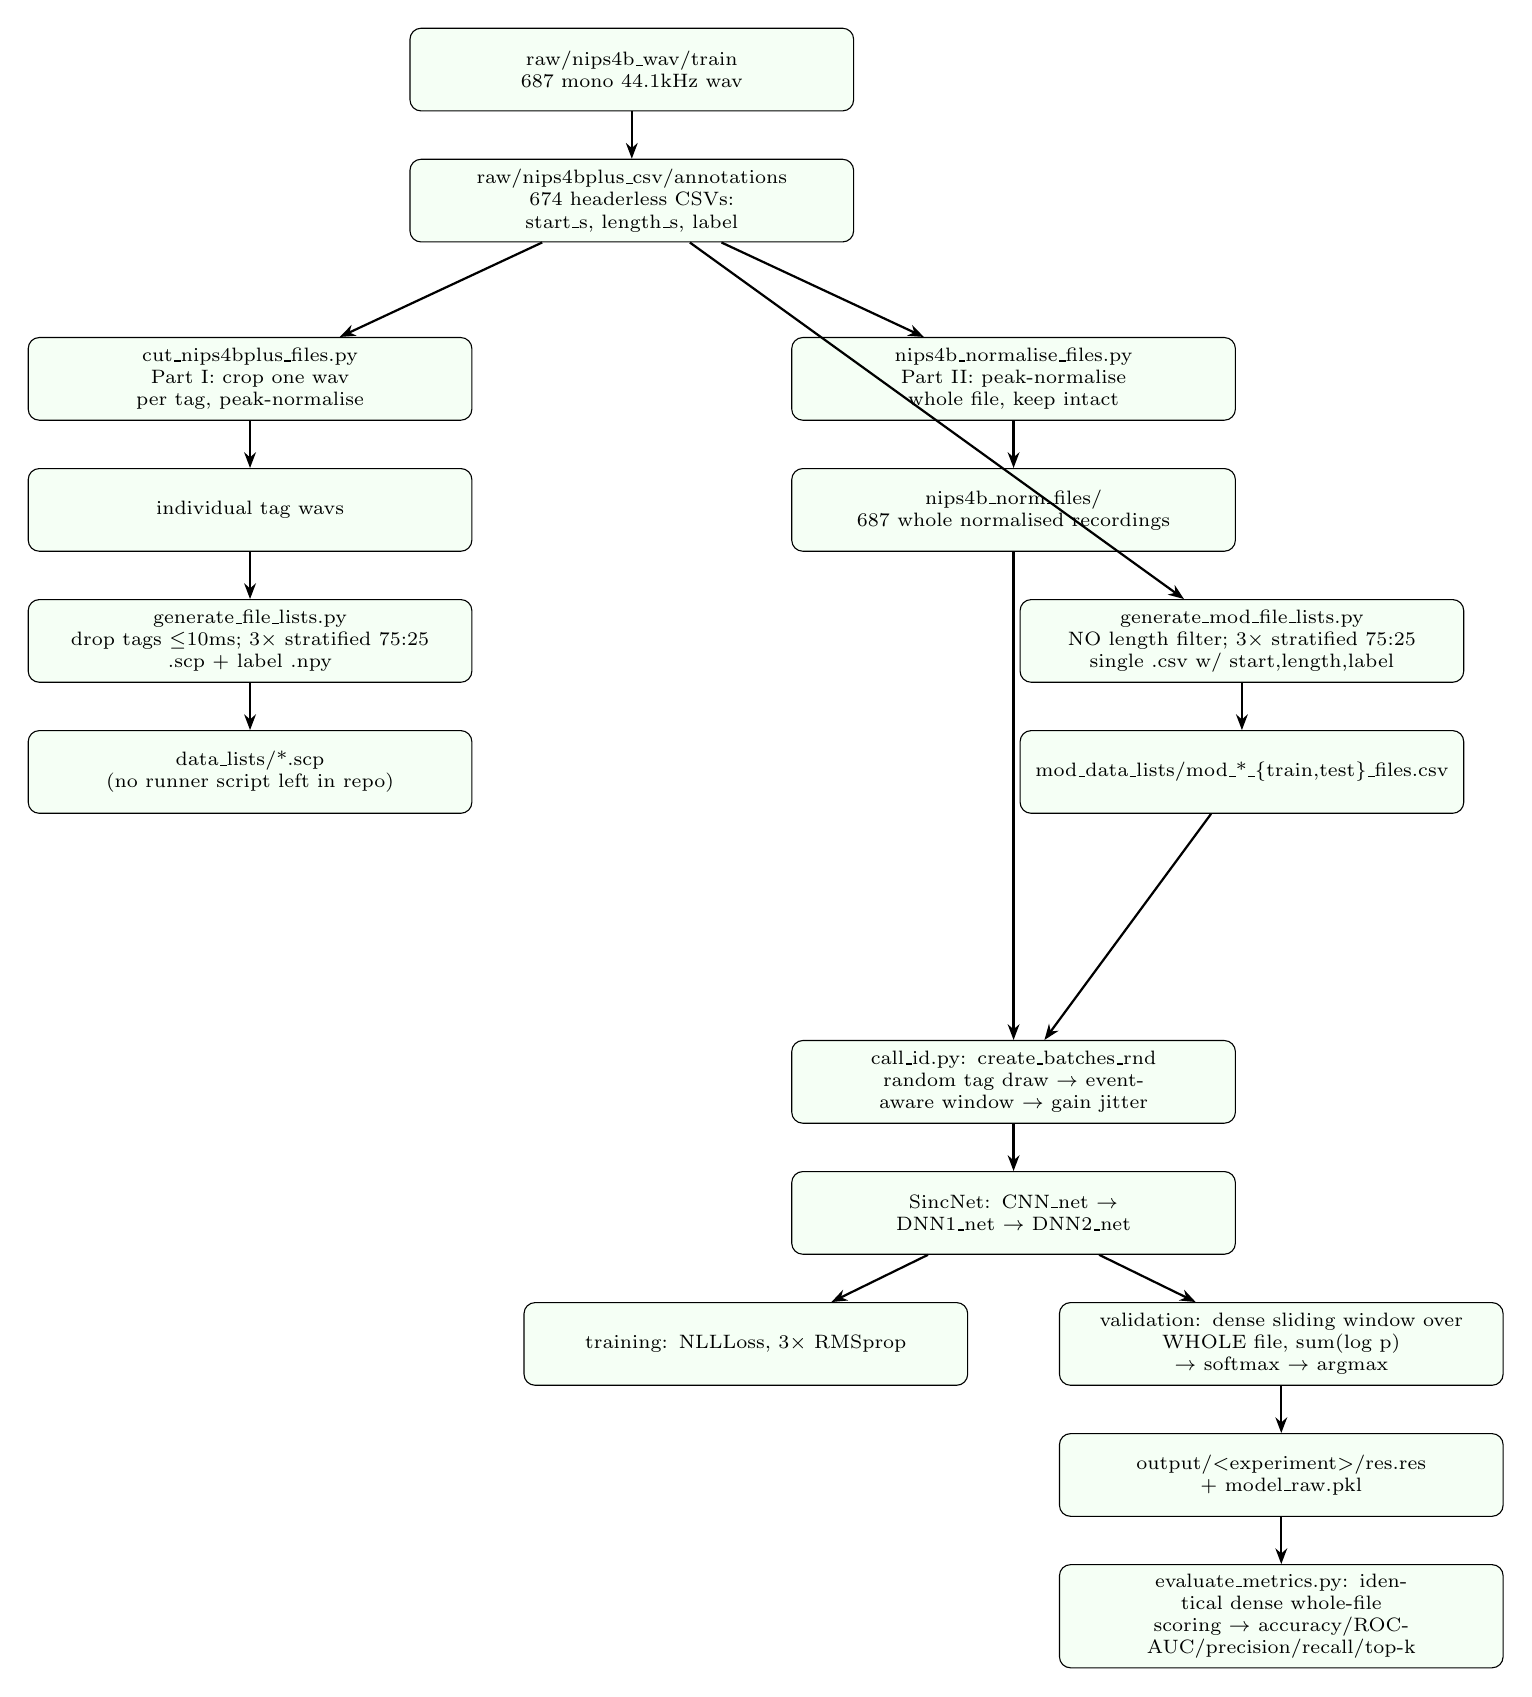
\begin{tikzpicture}[
  node distance=6mm and 10mm,
  box/.style={rectangle, draw, rounded corners, fill=green!4, align=center,
    text width=5.4cm, minimum height=1.05cm, font=\scriptsize},
  arr/.style={-{Stealth[length=2mm]}, thick}
]
\node[box] (a) {raw/nips4b\_wav/train\\687 mono 44.1kHz wav};
\node[box, below=of a] (b) {raw/nips4bplus\_csv/annotations\\674 headerless CSVs: start\_s, length\_s, label};

\node[box, below left=12mm and -8mm of b] (c1) {cut\_nips4bplus\_files.py\\Part I: crop one wav per tag, peak-normalise};
\node[box, below right=12mm and -8mm of b] (c2) {nips4b\_normalise\_files.py\\Part II: peak-normalise whole file, keep intact};

\node[box, below=of c1] (d1) {individual tag wavs};
\node[box, below=of c2] (d2) {nips4b\_norm\_files/\\687 whole normalised recordings};

\node[box, below=of d1] (e1) {generate\_file\_lists.py\\drop tags $\leq$10ms; 3$\times$ stratified 75:25\\.scp + label .npy};
\node[box, below=of d2, xshift=2.9cm] (e2) {generate\_mod\_file\_lists.py\\NO length filter; 3$\times$ stratified 75:25\\single .csv w/ start,length,label};

\node[box, below=of e1] (f1) {data\_lists/*.scp\\(no runner script left in repo)};
\node[box, below=of e2] (f2) {mod\_data\_lists/mod\_*\_\{train,test\}\_files.csv};

\node[box, below=of d2, yshift=-5.6cm] (g) {call\_id.py: create\_batches\_rnd\\random tag draw $\to$ event-aware window $\to$ gain jitter};
\node[box, below=of g] (h) {SincNet: CNN\_net $\to$ DNN1\_net $\to$ DNN2\_net};
\node[box, below=of h, xshift=-3.4cm] (i) {training: NLLLoss, 3$\times$ RMSprop};
\node[box, below=of h, xshift=3.4cm] (j) {validation: dense sliding window over\\WHOLE file, sum(log p) $\to$ softmax $\to$ argmax};
\node[box, below=of j] (k) {output/\textless experiment\textgreater/res.res + model\_raw.pkl};
\node[box, below=of k] (l) {evaluate\_metrics.py: identical dense whole-file\\scoring $\to$ accuracy/ROC-AUC/precision/recall/top-k};

\draw[arr] (a)--(b);
\draw[arr] (b)--(c1); \draw[arr] (b)--(c2);
\draw[arr] (c1)--(d1); \draw[arr] (c2)--(d2);
\draw[arr] (d1)--(e1); \draw[arr] (b) -- (e2);
\draw[arr] (e1)--(f1); \draw[arr] (e2)--(f2);
\draw[arr] (d2)--(g); \draw[arr] (f2)--(g);
\draw[arr] (g)--(h);
\draw[arr] (h)--(i); \draw[arr] (h)--(j);
\draw[arr] (j)--(k); \draw[arr] (k)--(l);
\end{tikzpicture}}
\caption{The full data pipeline. Left branch (Part I) is present but not
consumed by any surviving trainer in this checkout; right branch (Part II)
is what every result actually traces back to.}
\label{fig:pipeline}
\end{figure}

\subsection{Algorithmic breakdown, with complexity}
\label{sec:C2}

\textbf{1. Amplitude normalisation}, per file, $O(N)$ in file length $N$:
\begin{lstlisting}
signal <- float64(signal)
signal <- signal / |max(signal)|
\end{lstlisting}

\textbf{2. List generation / splitting}, whole corpus:
\begin{lstlisting}
for each non-empty annotation CSV (674 files):
    for each row:
        (type, scientific) <- lookup(label, species_table)      # O(1)
        if type resolved: append {file, type, class, species, start, length, label}
# O(5,775) total rows built
for each of 3 class schemes:
    train, test <- stratified_split(rows_for_scheme, test_size=0.25)  # O(n log n)
    write CSV
\end{lstlisting}
No \texttt{random\_state} $\Rightarrow$ this step is \textbf{non-deterministic
across runs} (Section~\ref{sec:B4}).

\textbf{3. Training-time sampling}, per minibatch of size $B$:
\begin{lstlisting}
for i in 1..B:
    row <- uniform_random(tag_table, with_replacement=True)         # O(1)
    signal <- sf.read(file_for(row))                # O(file length) DISK READ, every call
    window <- event_aware_crop(signal, row.start, row.length, wlen) # O(wlen)
    batch[i] <- window * Uniform(0.8, 1.2)
\end{lstlisting}
For the enhanced Bird-Species config ($N_{\text{batches}}=80$,
$\text{batch}=128$, $N_{\text{epochs}}=400$), this is
$80\times128\times400=4{,}096{,}000$ full \texttt{sf.read()} calls against a
687-file, $\sim$36-minute corpus over one training run --- \textbf{no
caching of decoded audio} across draws or epochs, making the training loop
I/O-bound by construction.

\textbf{4. Dense whole-file evaluation}, per test row:
\begin{lstlisting}
signal <- sf.read(file_for(row))                    # re-read even if already scored this file
N_fr   <- floor((len(signal) - wlen) / wshift)       # e.g. (220500-705)/44 ~ 4,995 frames
pout[0..N_fr] <- forward(model, each of N_fr overlapping windows)   # O(N_fr) forward passes
score  <- softmax(sum(pout, axis=0))
pred   <- argmax(score)
\end{lstlisting}
Because 1,320 bird-species test rows resolve to only 417 unique files,
\textbf{903 of 1,320 per-row evaluations (68\%) re-run an identical dense
whole-file forward pass} already computed for an earlier row referencing the
same file --- evaluation cost scales with \emph{tag count}, not
\emph{unique-file count}, with no memoisation.

\subsection{Missing values, feature scaling, class imbalance --- as implemented}
\label{sec:C3}

\textbf{Missing values.} There is no tabular ``NaN cell'' in this pipeline,
but there is a direct structural analogue: an annotation record can be
(a)~\textbf{present with $\geq 1$ rows} (569 files --- the normal case),
(b)~\textbf{present but empty} (105 files --- a bare CRLF; the annotator
reviewed the file and found nothing --- \emph{informative} missingness, ``
confirmed zero,'' not ``unknown''), or (c)~\textbf{absent entirely} (13
files --- genuinely undocumented, ``we don't know''). \textbf{The
pipeline's handling is implicit listwise deletion}: both (b) and (c)
contribute zero rows to the tag table, with no imputation, no explicit
``unknown'' class, and \textbf{no code path that distinguishes ``confirmed
empty'' from ``we don't know''} even though these have different epistemic
status.

\textbf{Feature scaling.} In the conventional ML sense (per-feature
standardisation of a tabular design matrix) there is \textbf{none}, because
the input is not a feature matrix --- it is the raw signal itself
(Section~\ref{sec:A3}). The only scaling operation present is the per-file
peak-amplitude normalisation (Section~\ref{sec:B31}), plus the online
multiplicative jitter applied per training draw. No z-scoring, min-max
scaling, or log-compression of amplitude is applied anywhere, despite
Part A's evidence that amplitude features in this corpus are lognormally
distributed with extreme kurtosis.

\textbf{Class imbalance.} \textbf{Not handled anywhere in the modelling
pipeline.} \texttt{create\_batches\_rnd} draws tag rows \textbf{uniformly at
random}, so a class with 282 instances (\texttt{Sylcan\_song}) is
$\sim$30$\times$ more likely to appear in any given minibatch than a class
with 9 (\texttt{Cicatr\_song}) --- the raw corpus's Zipf-like imbalance
(Section~\ref{sec:A54}) propagates directly, unmodified, into
gradient-update frequency per class. \texttt{nn.NLLLoss()} is instantiated
with no \texttt{weight} argument, so the loss itself applies no per-class
re-weighting either. There is no weighted sampler, no oversampling of
minority tags, no undersampling of majority tags, and no focal-loss-style
down-weighting anywhere in the training script.

\subsection{A better pipeline, theoretically justified}
\label{sec:C4}

Each item below is tied to a specific measurement from Part A/B, stated as a
design option, not a change made to this codebase.

\begin{table}[h]
\centering
\small
\begin{tabularx}{\textwidth}{Y Y}
\toprule
Issue (measured) & Theoretically justified alternative \\
\midrule
4.1M redundant \texttt{sf.read()} calls/run (Sec.~\ref{sec:C2}) & Decode once into an in-memory (or memory-mapped) array per file at startup; converts an I/O-bound loop into a compute-bound one \\
68\% redundant whole-file forward passes at eval (Sec.~\ref{sec:C2}) & Memoise the dense per-file score vector keyed by filename; compute once per unique file (417, not 1{,}320) \\
Uniform-random sampling into a Zipf-imbalanced target (Sec.~\ref{sec:C3}) & \texttt{WeightedRandomSampler} with per-tag weight $\propto 1/n_{\text{class}}$ (or $1/\sqrt{n_{\text{class}}}$), or class-weighted \texttt{NLLLoss} \\
Peak (signed-max) normalisation on lognormal, kurtotic amplitude (Sec.~\ref{sec:B31}) & RMS-based or log-compressive per-file scaling; at minimum normalise by $\max(|\text{signal}|)$ \\
Tag-level, unseeded split $\Rightarrow$ 96.5\% file-level leakage (Sec.~\ref{sec:A7}, \ref{sec:B4}) & Group-aware split (\texttt{GroupShuffleSplit}/\texttt{GroupKFold} keyed on source filename) with a fixed \texttt{random\_state} \\
Zero dropout, measured train/test gap (Sec.~\ref{sec:B38}) & Non-zero FC dropout and/or weight decay \\
Best-of-N selection against the reported test set (Sec.~\ref{sec:B5}) & Three-way train/validation/test split; test touched once for the final number \\
Whole-file evaluation scores a different task than stated (Sec.~\ref{sec:A7}) & Restrict scoring to frames overlapping the tag's own span, matching the paper's stated methodology \\
No LR schedule over 32{,}000--160{,}000 steps (Sec.~\ref{sec:B310}) & Cosine or step decay on top of the existing RMSprop optimizers \\
\bottomrule
\end{tabularx}
\end{table}

\placeholderfig{a physical schematic/photograph of the SM2BAT + SMX-US
microphone deployment described in the papers' methods (bat-echolocation
recorders opportunistically also capturing birdsong, 6~dB SNR trigger, 2~s
window). Purely descriptive hardware information, not derivable from the
released audio or annotation files.}{Placeholder --- field recording
hardware schematic (source: Morfi et al.\ 2019 / Bravo Sanchez et al.\ 2021,
Methods).}

\subsection{Closing scorecard}

The pipeline is internally consistent and each individual step has a
traceable rationale once cross-referenced against the dataset's actual
measured statistical shape (Part A) --- this is a genuinely well-motivated
system, not an arbitrary one. Its two largest, most consequential gaps as
\emph{implemented} (not as \emph{described} in the paper's text) are
(1)~a train/test split that leaks recording-level context across the
boundary at the unit-of-splitting level, and (2)~a training/evaluation loop
with no mechanism --- sampling, loss weighting, or regularisation --- that
responds to the corpus's own measured, Zipf-shaped class imbalance. Both
are diagnosable directly from the EDA in Part A without reference to the
paper's reported numbers at all.

\end{document}
